\chapter{\posl{} Class diagrams}
\label{app:diag}
\textit{In this appendix are presented the class diagrams of the current implementation of \posl\footnote{\posl's source code is abailable at \href{https://github.com/alejandro-reyesamaro/POSL}{https://github.com/alejandro-reyesamaro/POSL}}. In these diagrams are shown only the most important classes (and fields) that were used during the experimentation process for this thesis, in order to facilitate the understanding of the class design.}
\vfill
\newpage


%\noindent\rule[2pt]{\textwidth}{0.8pt}

\clearpage

%\begin{figure}
%	\centering
%	\subfloat[][Data \opch]{
%		\label{subfig:doch}
%		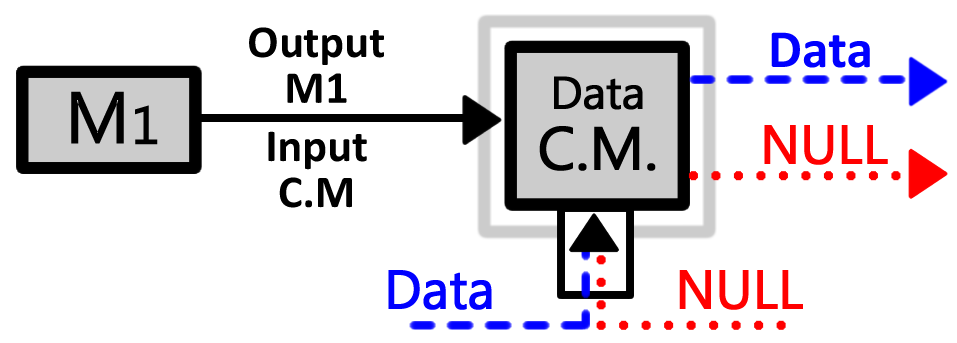
\includegraphics[width=0.4\linewidth]{D_OCh.png}
%	}
%	\hspace{0.05\textwidth}%
%	\subfloat[][Object \opch]{%
%		\label{subfig:ooch}
%		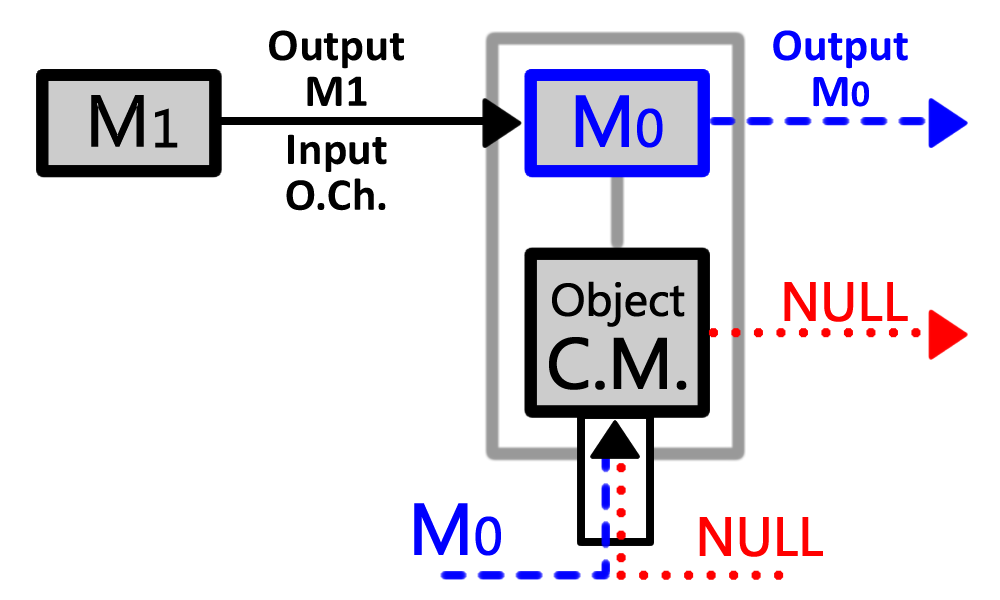
\includegraphics[width=0.4\linewidth]{O_OCh.png}
%	}
%	\caption[]{Communication module}
%	\label{fig:och}
%\end{figure}

\begin{figure}
	\centering
	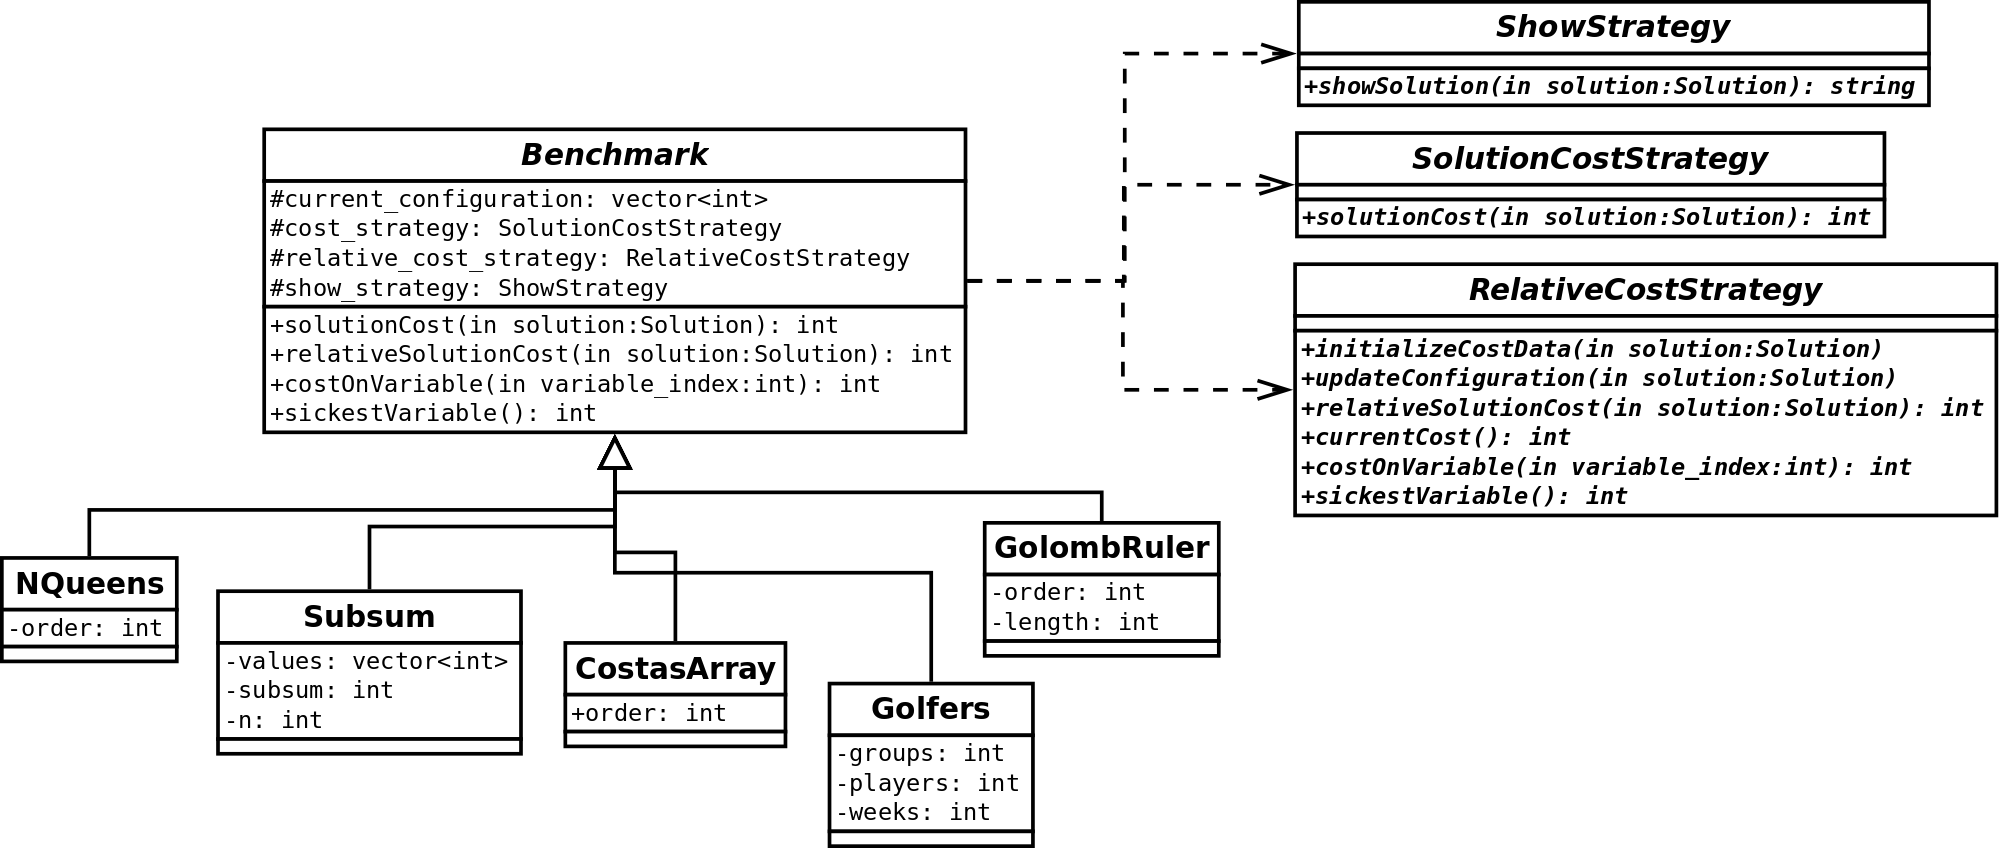
\includegraphics[width=\linewidth]{diabench.png}
	\caption[]{Benchmark class diagram}\label{diag:bench}
\end{figure}

\begin{figure}
	\centering
	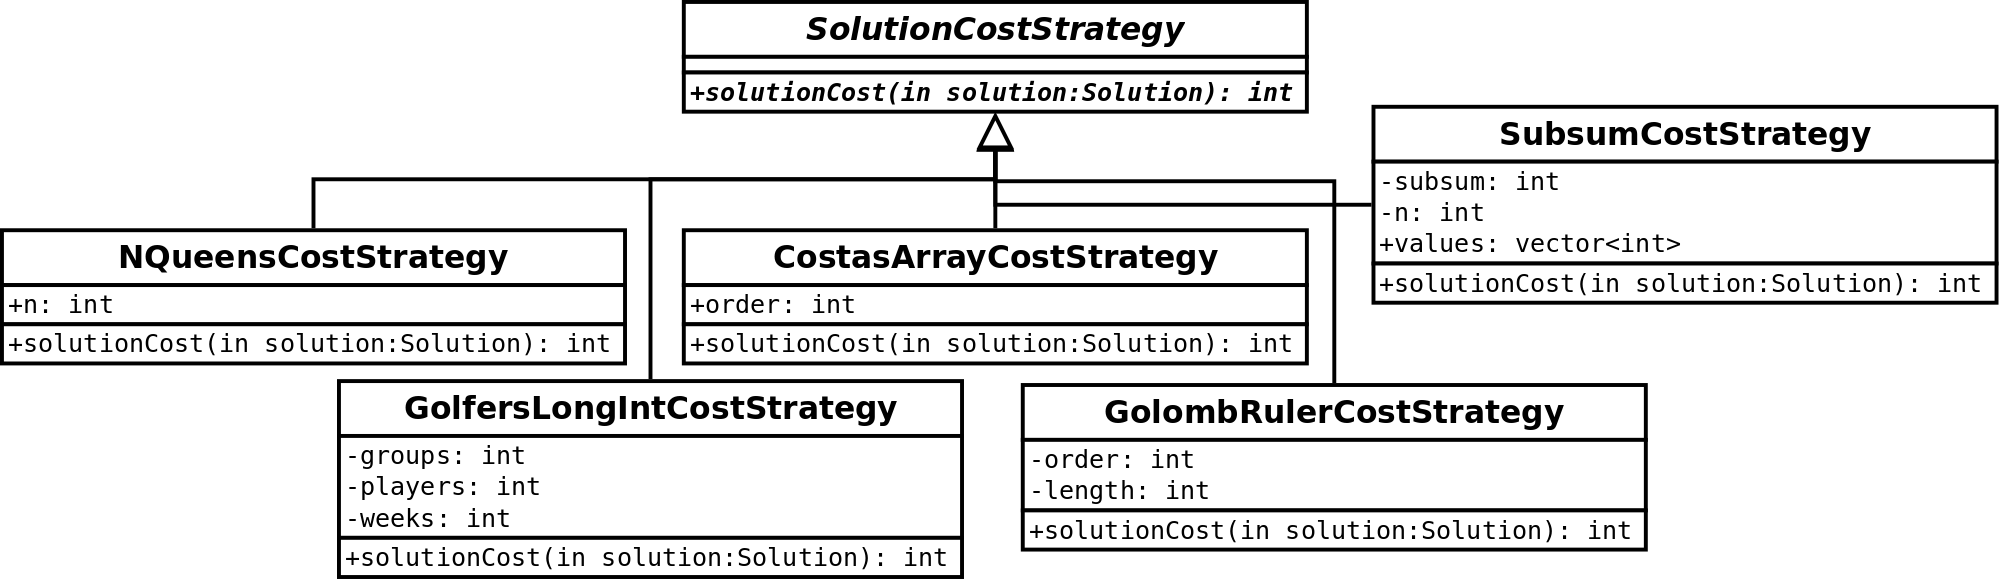
\includegraphics[width=\linewidth]{diacoststr.png}
	\caption[]{Cost strategy class diagram}\label{diag:coststr}
\end{figure}

\begin{figure}
	\centering
	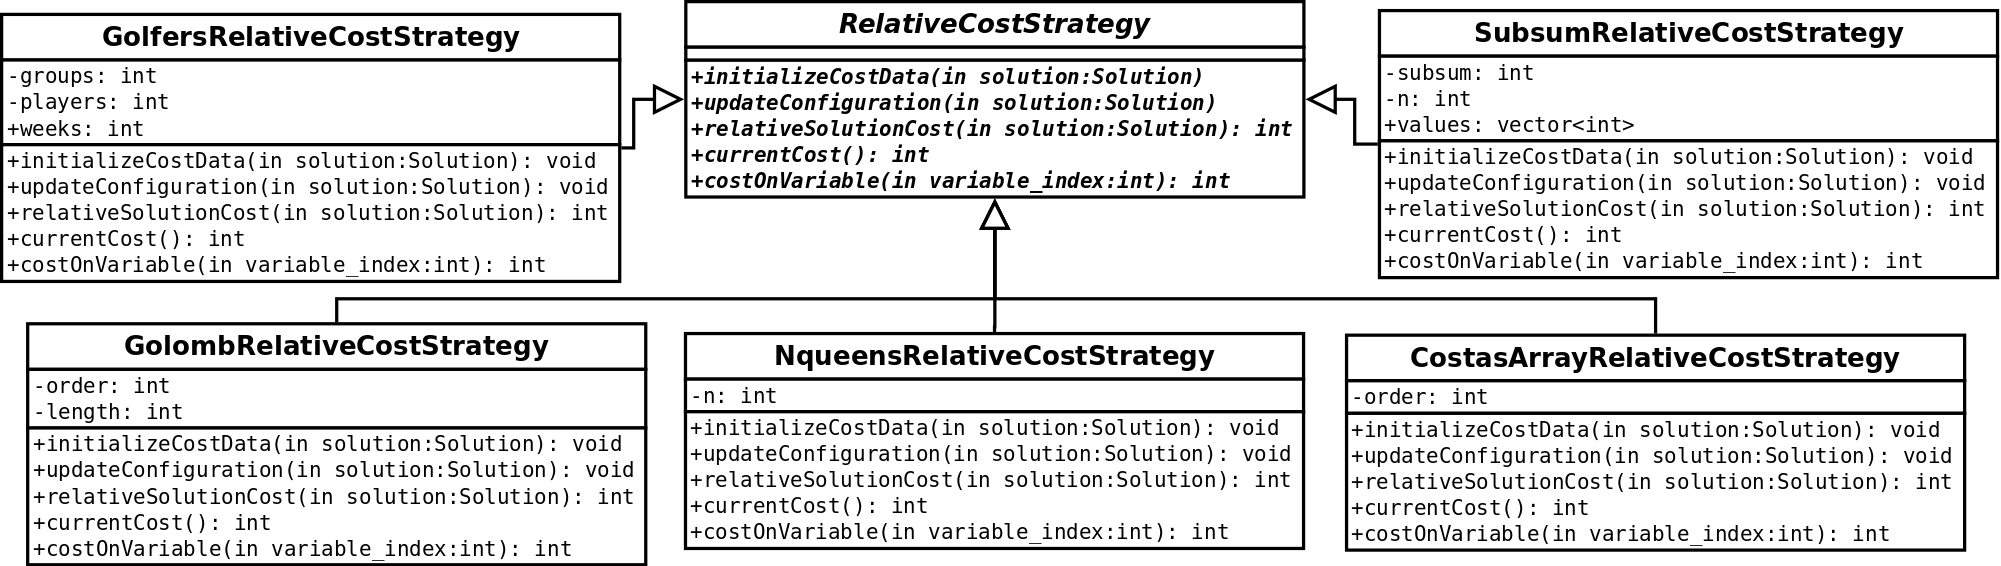
\includegraphics[width=\linewidth]{diarelacoststr.png}
	\caption[]{Relative cost strategy class diagram}\label{diag:relacoststr}
\end{figure}

\begin{figure}
	\centering
	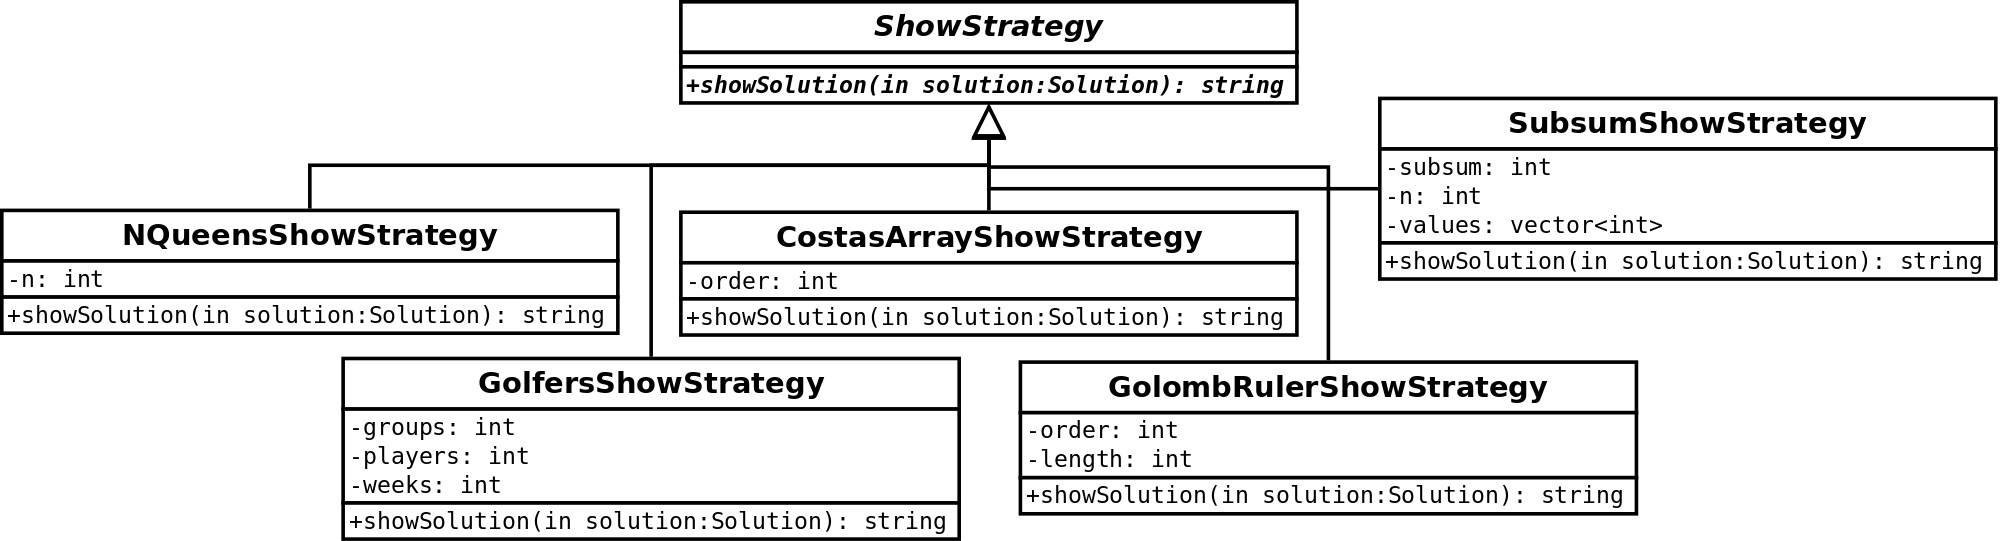
\includegraphics[width=\linewidth]{diashowstr.png}
	\caption[]{Show solution strategy class diagram}\label{diag:showstr}
\end{figure}

\begin{figure}
	\centering
	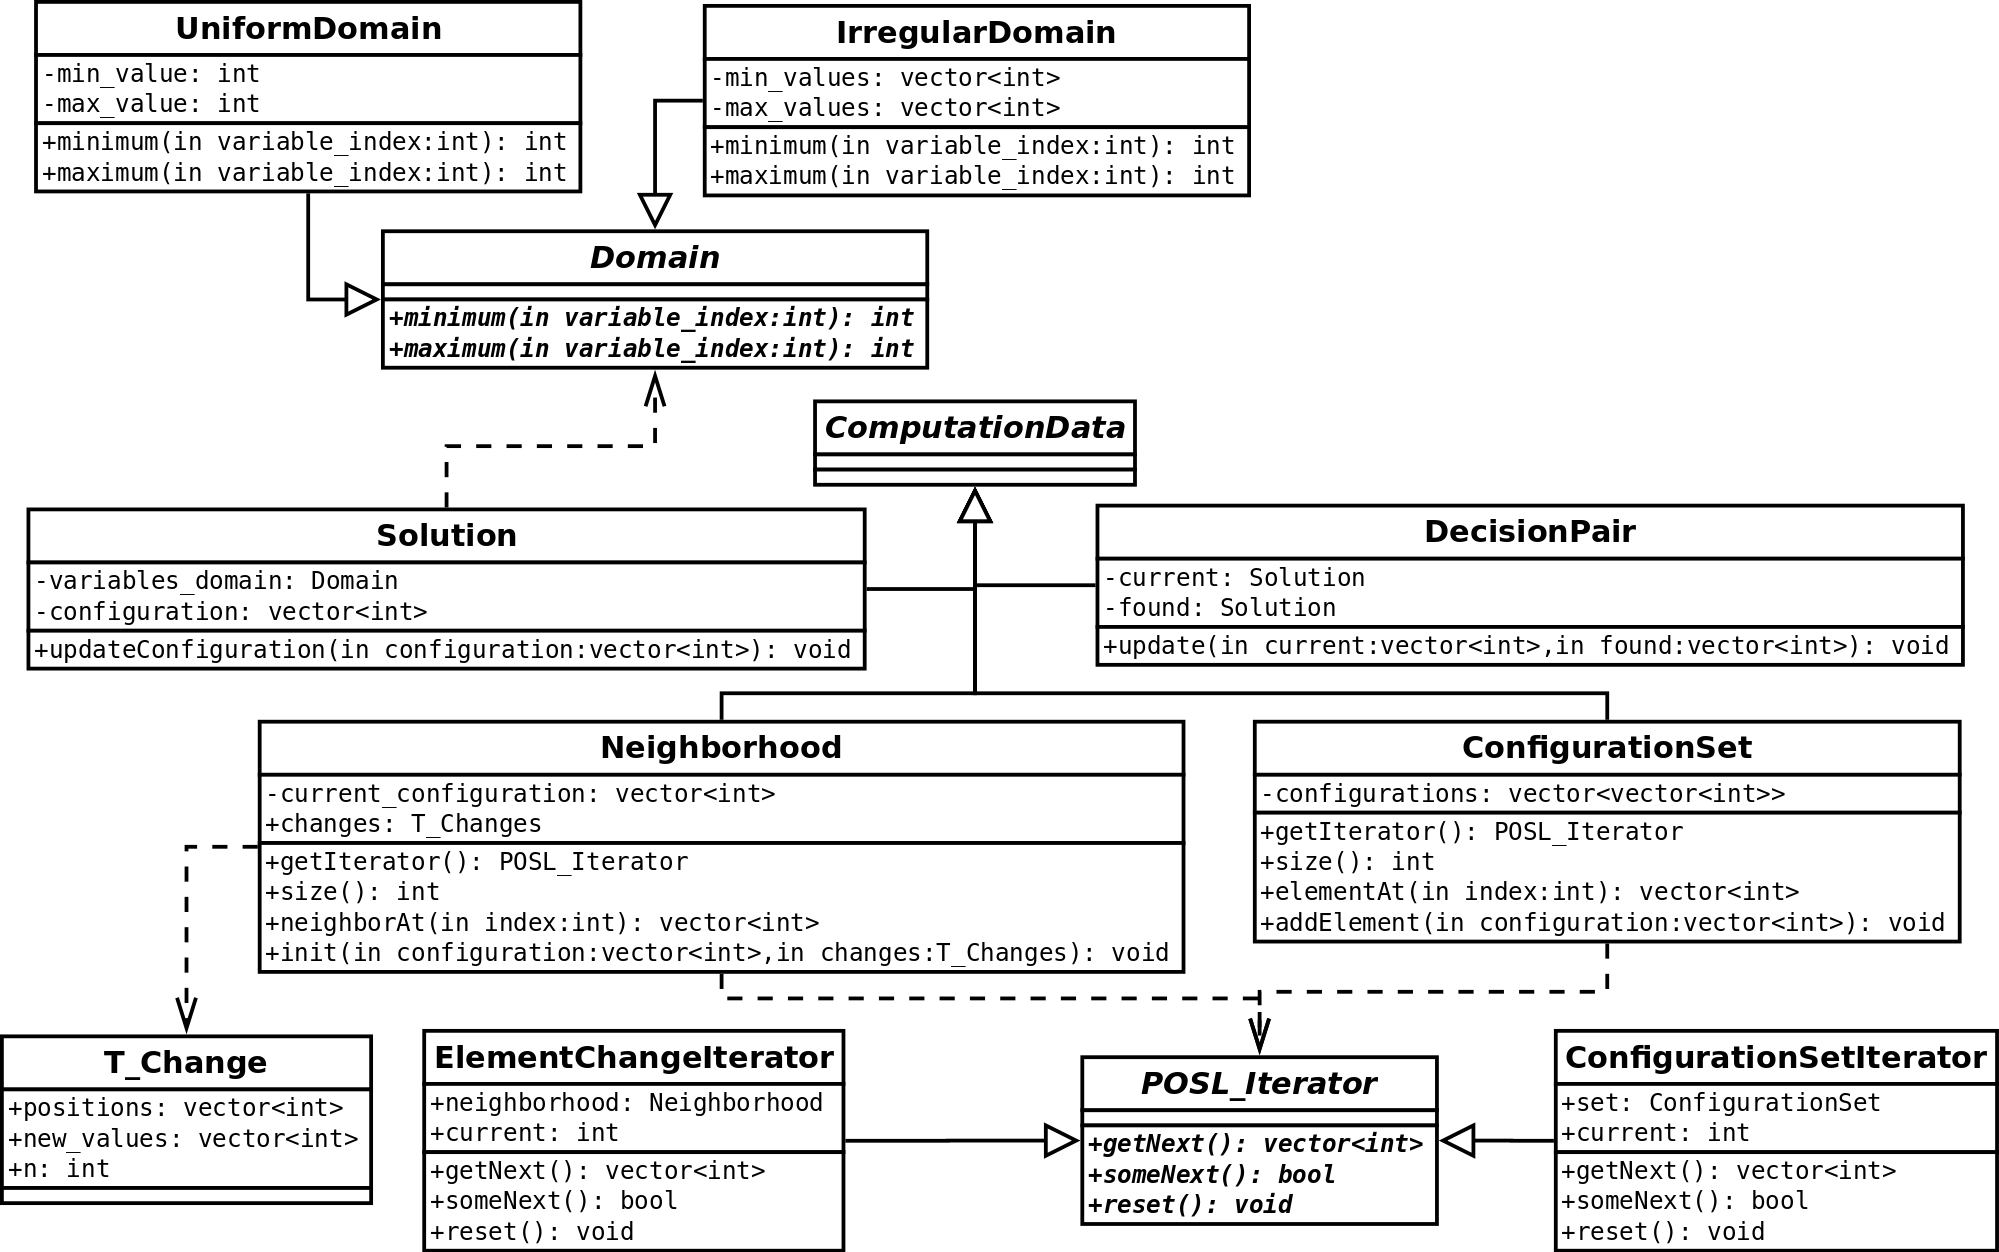
\includegraphics[width=\linewidth]{diadata.png}
	\caption[]{\posl{} data class diagram}\label{diag:data}
\end{figure}

\begin{figure}
	\centering
	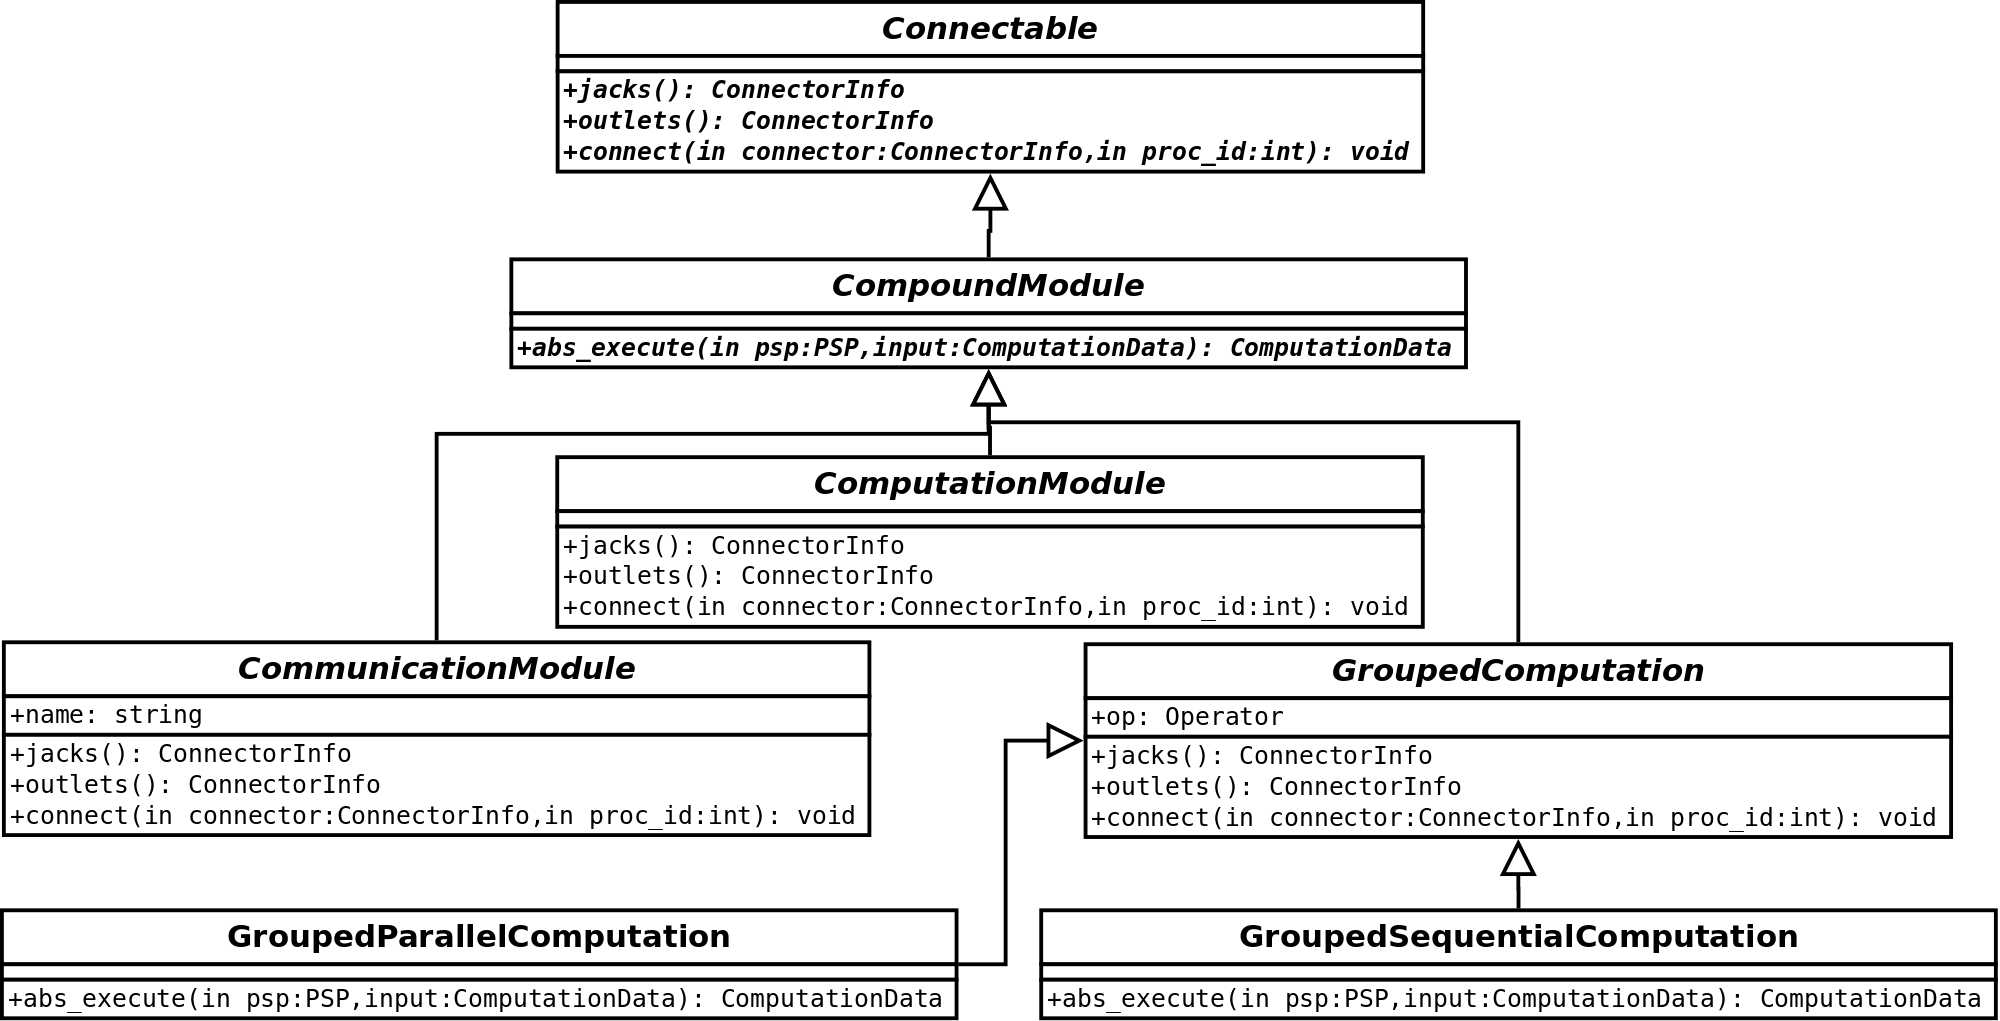
\includegraphics[width=\linewidth]{diacm.png}
	\caption[]{Compound modules class diagram}\label{diag:cm}
\end{figure}

\begin{figure}
	\centering
	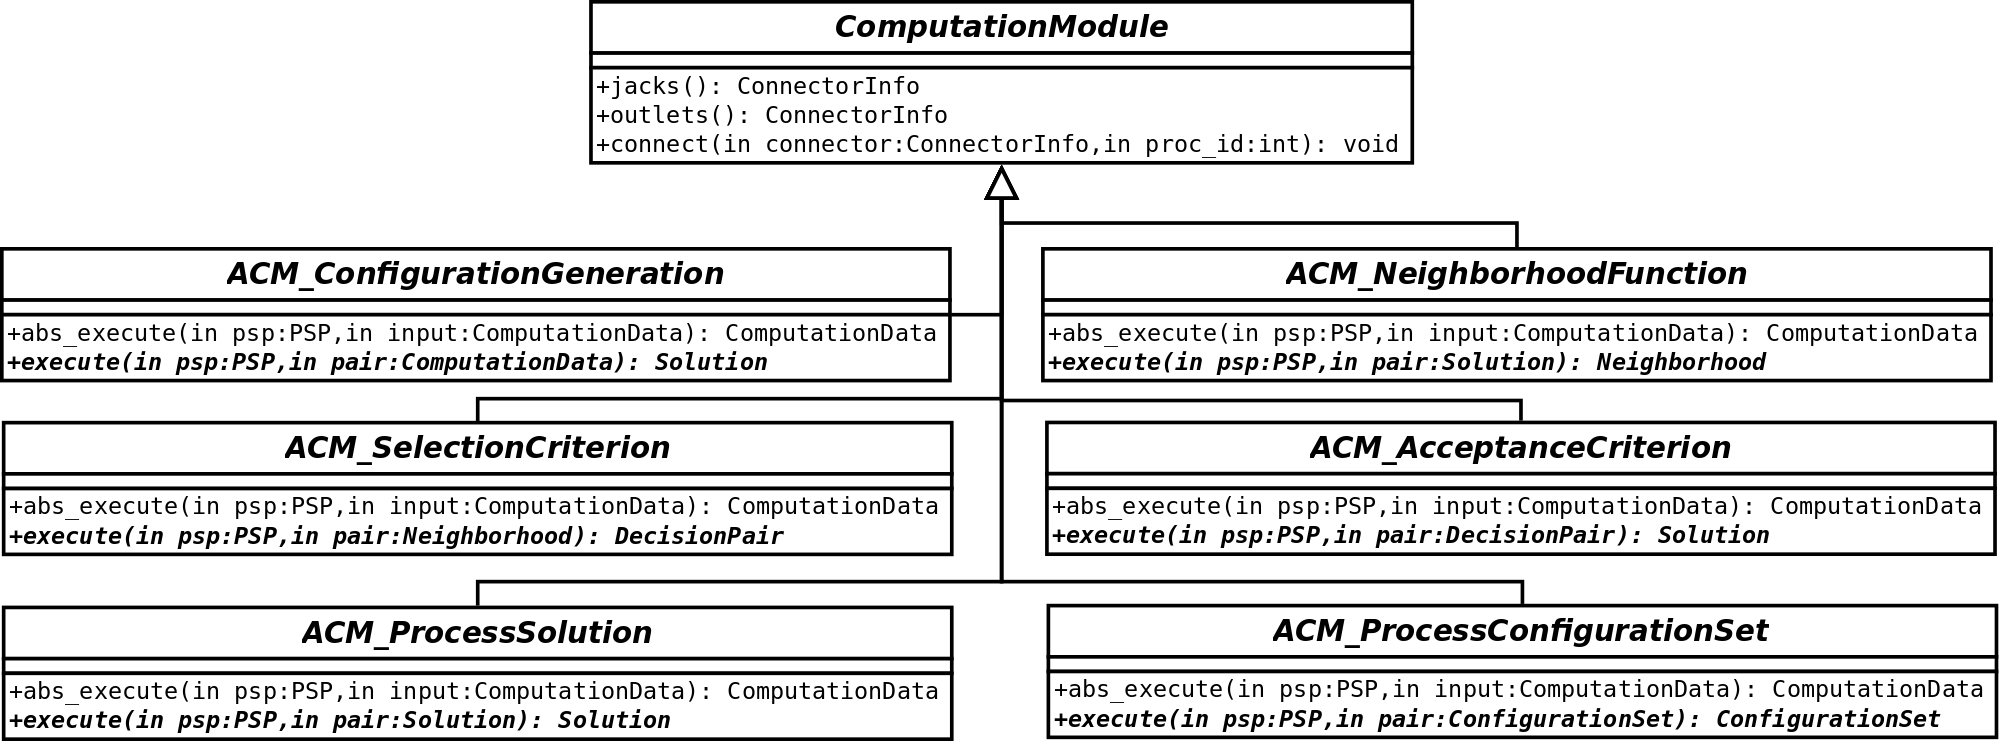
\includegraphics[width=\linewidth]{diaom.png}
	\caption[]{Abstract computation modules class diagram}\label{diag:om}
\end{figure}

\begin{figure}
	\centering
	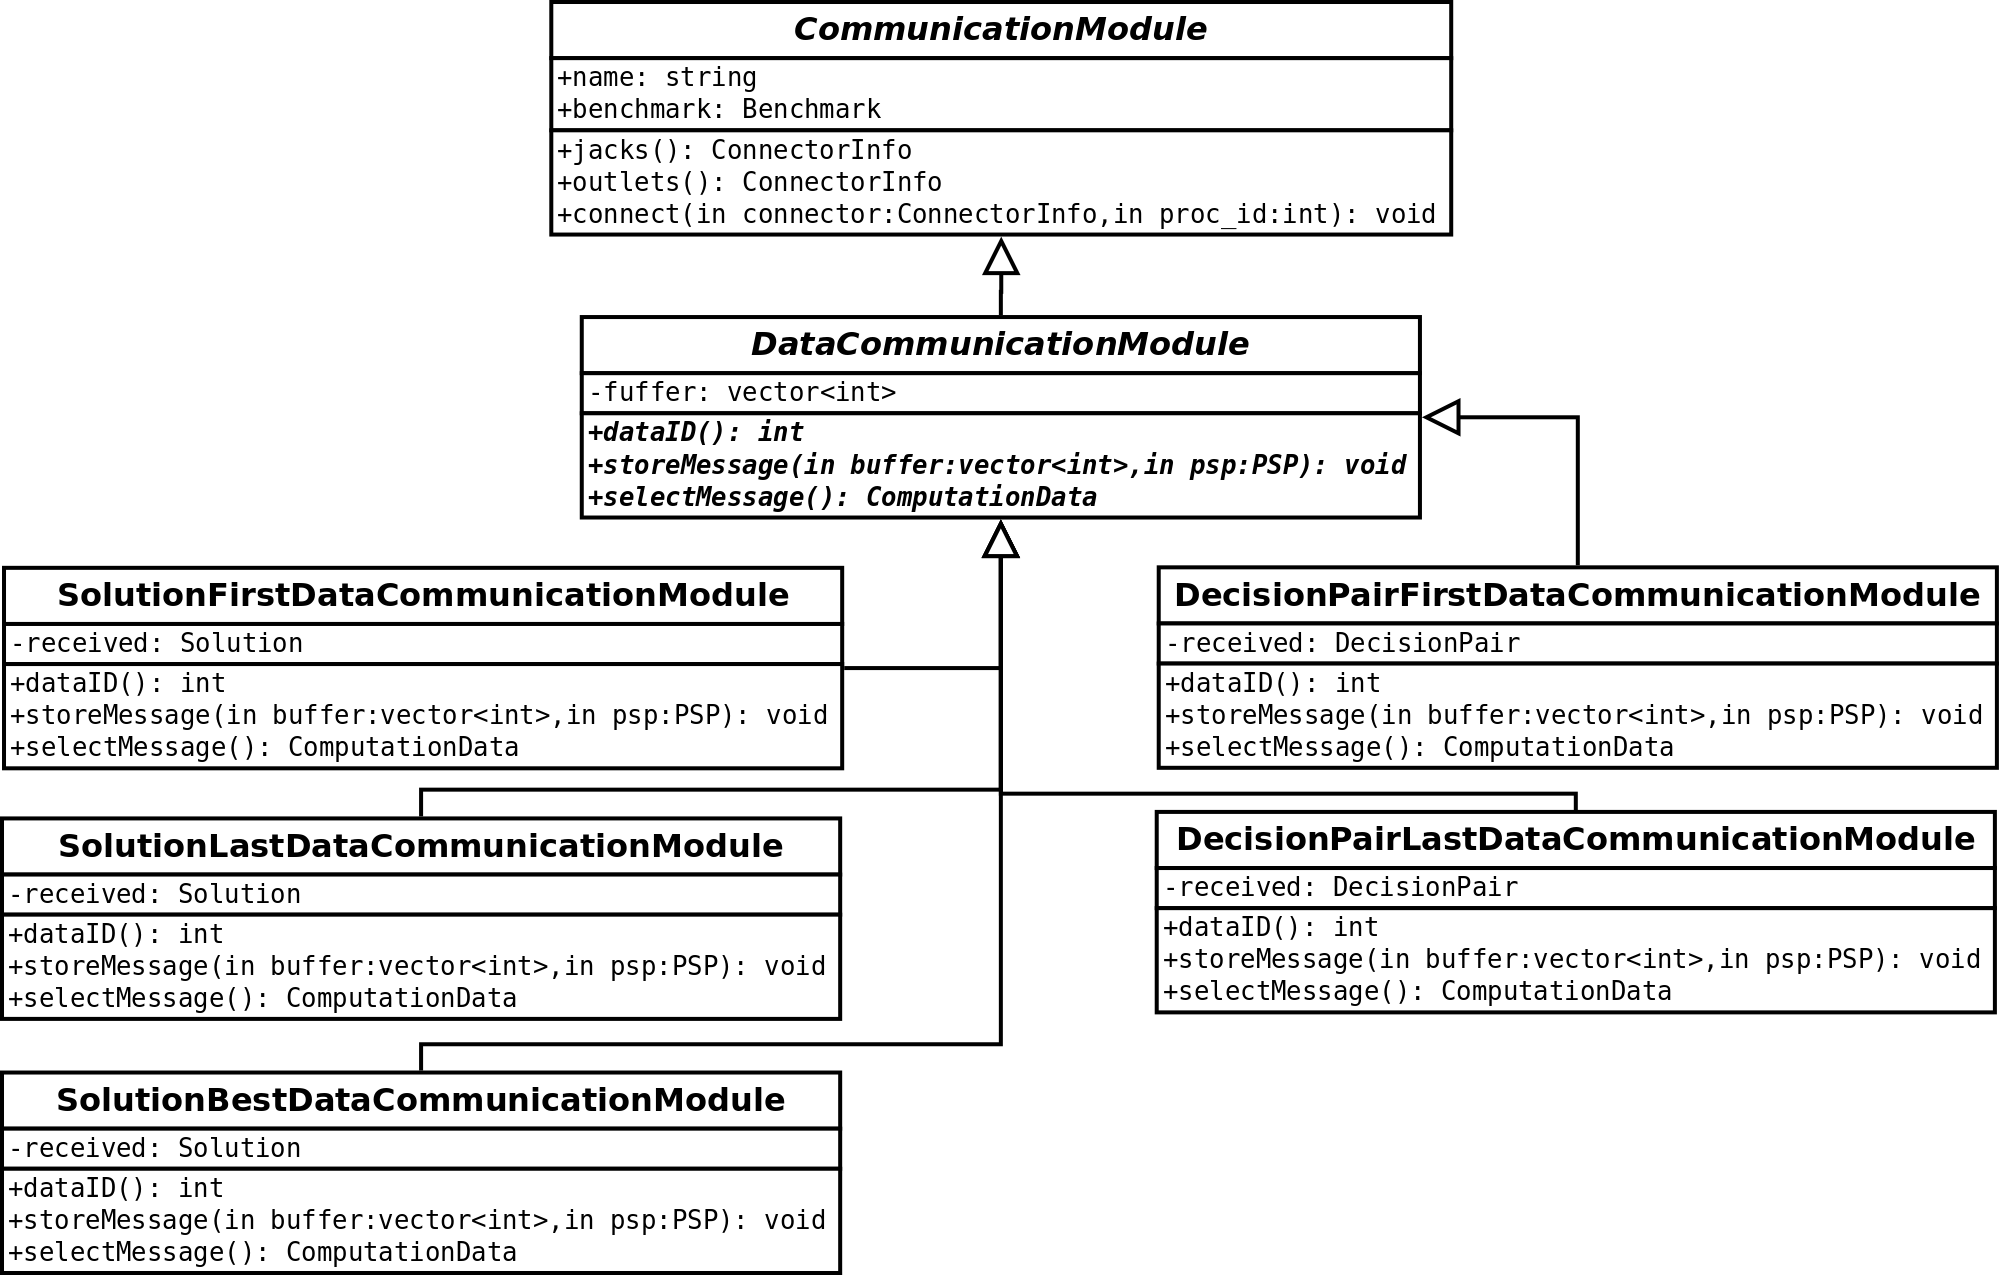
\includegraphics[width=\linewidth]{diaoch.png}
	\caption[]{Communication modules class diagram}\label{diag:opch}
\end{figure}

\begin{figure}
	\centering
	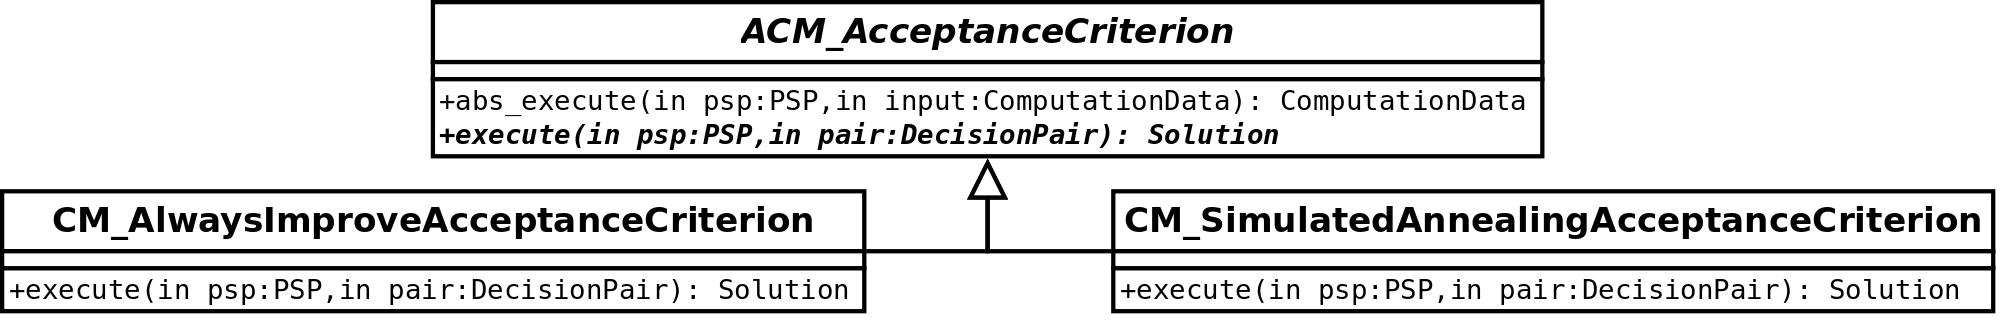
\includegraphics[width=\linewidth]{diaaomacc.png}
	\caption[]{Acceptance computation modules class diagram}\label{diag:accmodules}
\end{figure}

\begin{figure}
	\centering
	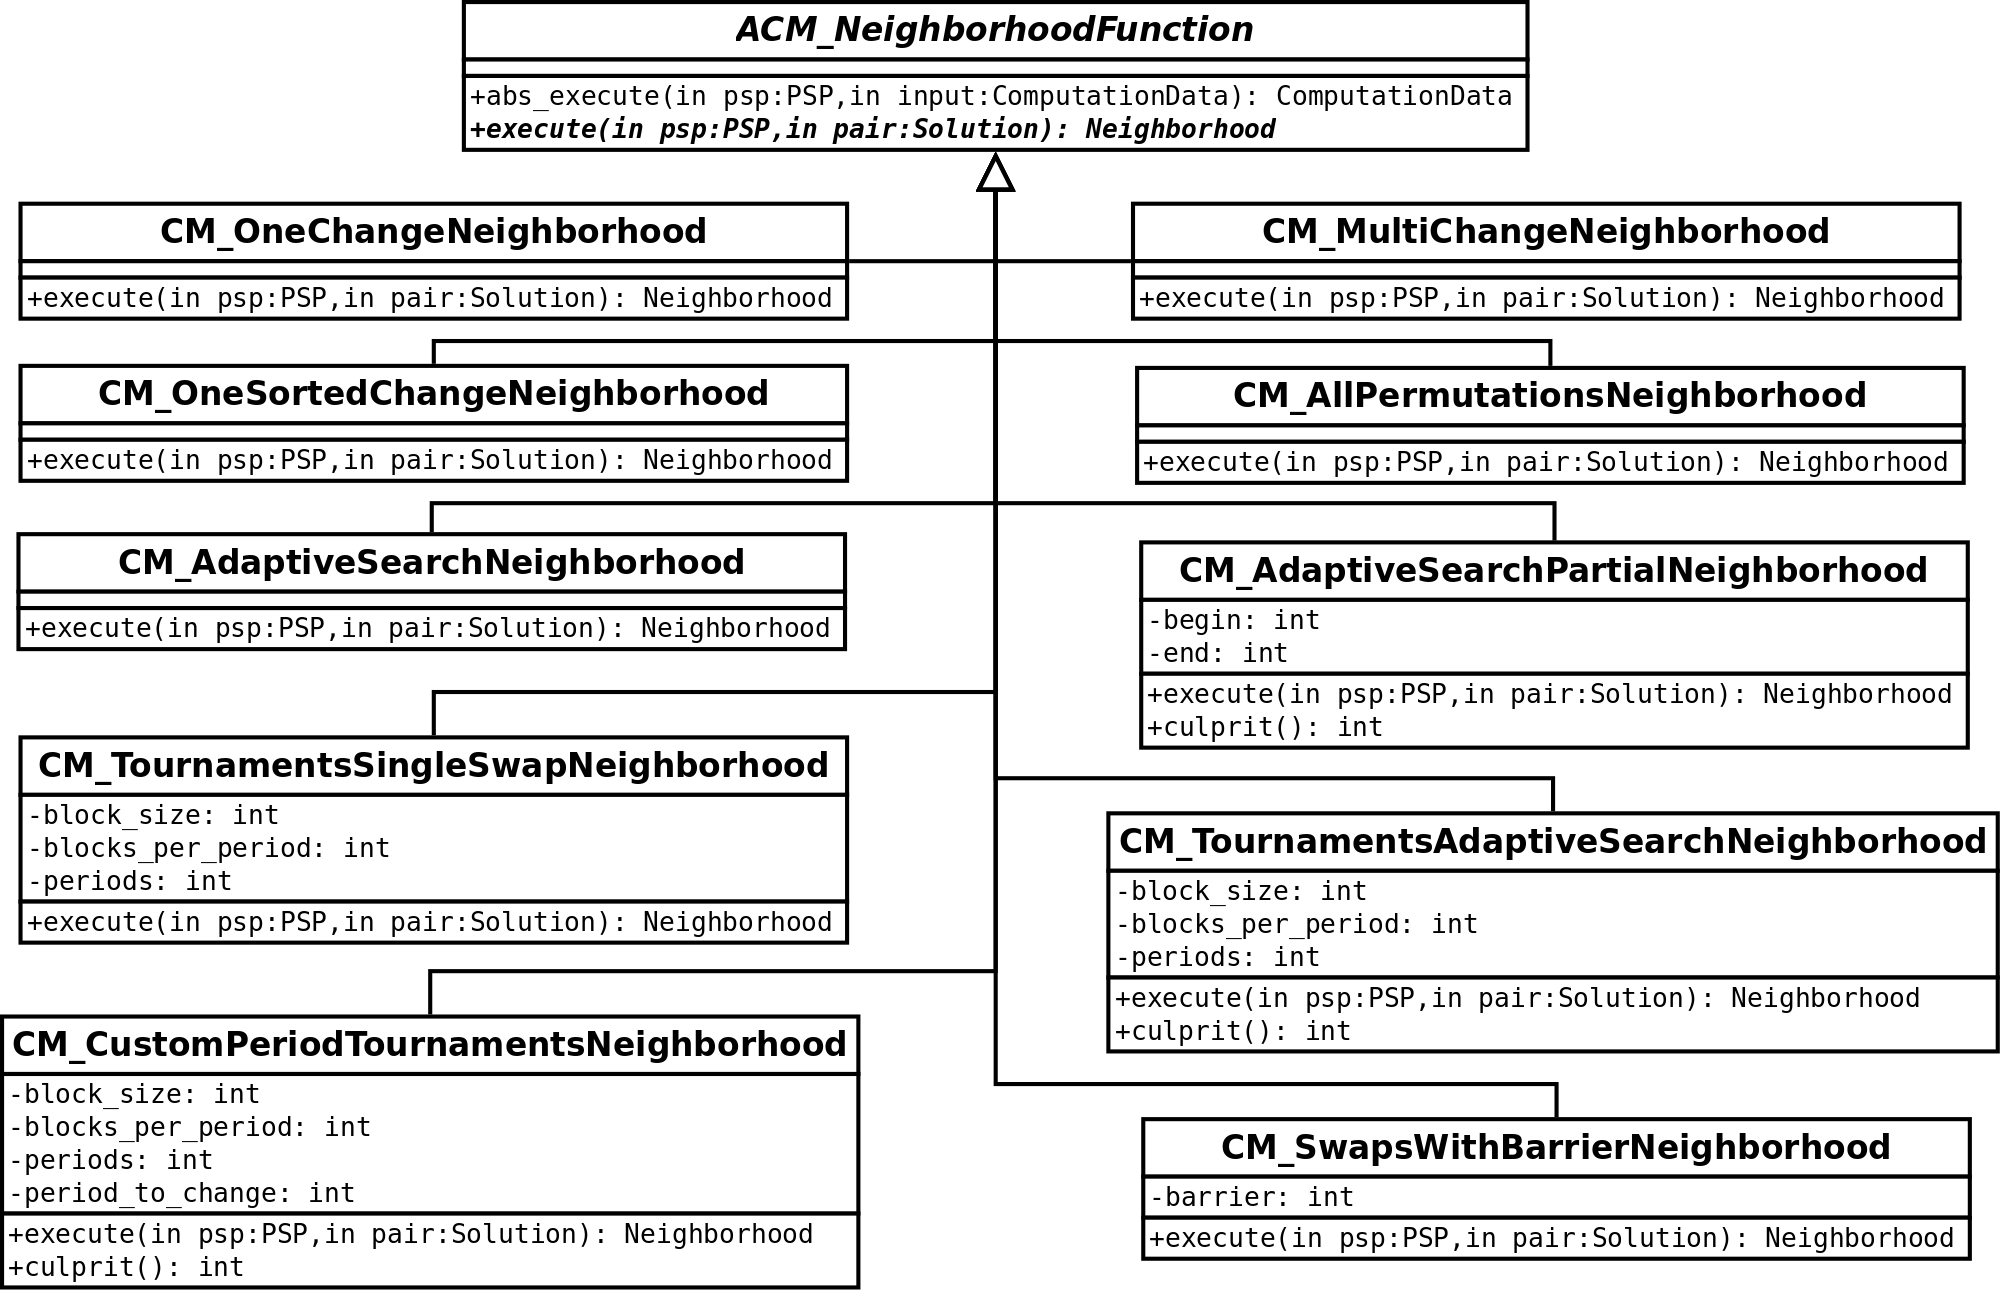
\includegraphics[width=\linewidth]{diaaomneigh.png}
	\caption[]{Neighborhood computation modules class diagram}\label{diag:neighmodules}
\end{figure}

\begin{figure}
	\centering
	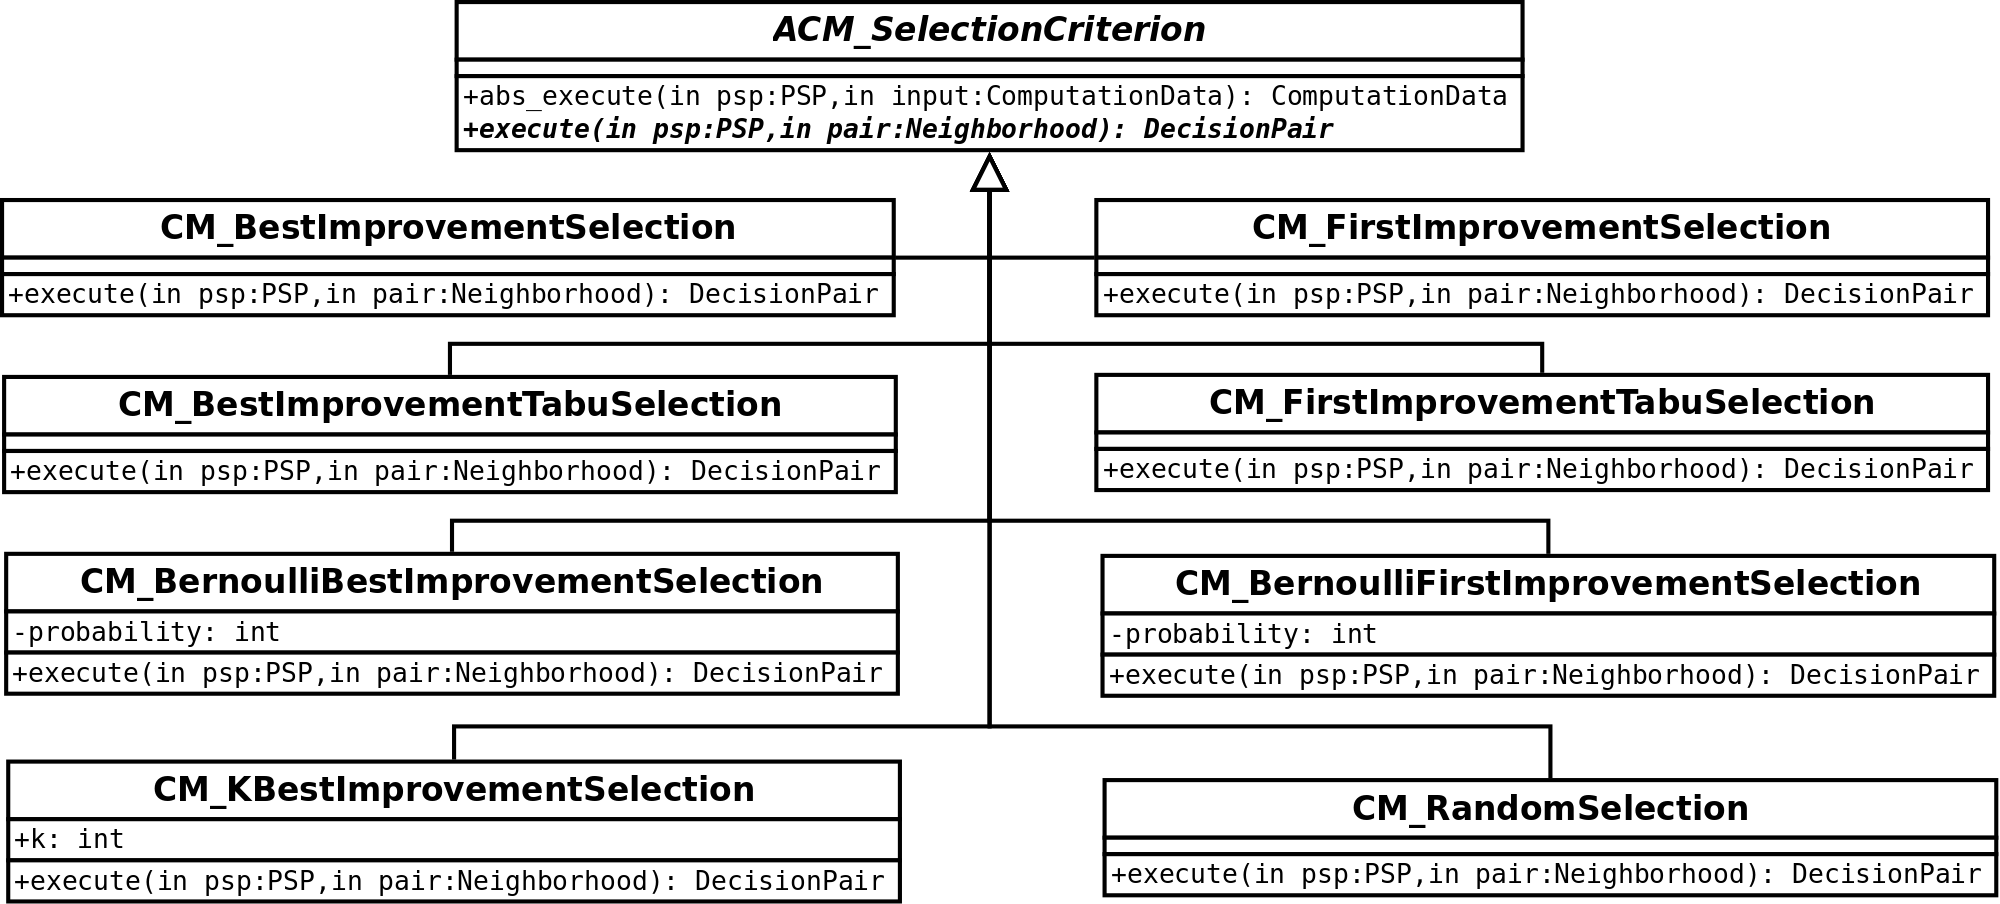
\includegraphics[width=\linewidth]{diaaomselect.png}
	\caption[]{Selection computation modules class diagram}\label{diag:selectmodules}
\end{figure}

\begin{figure}
	\centering
	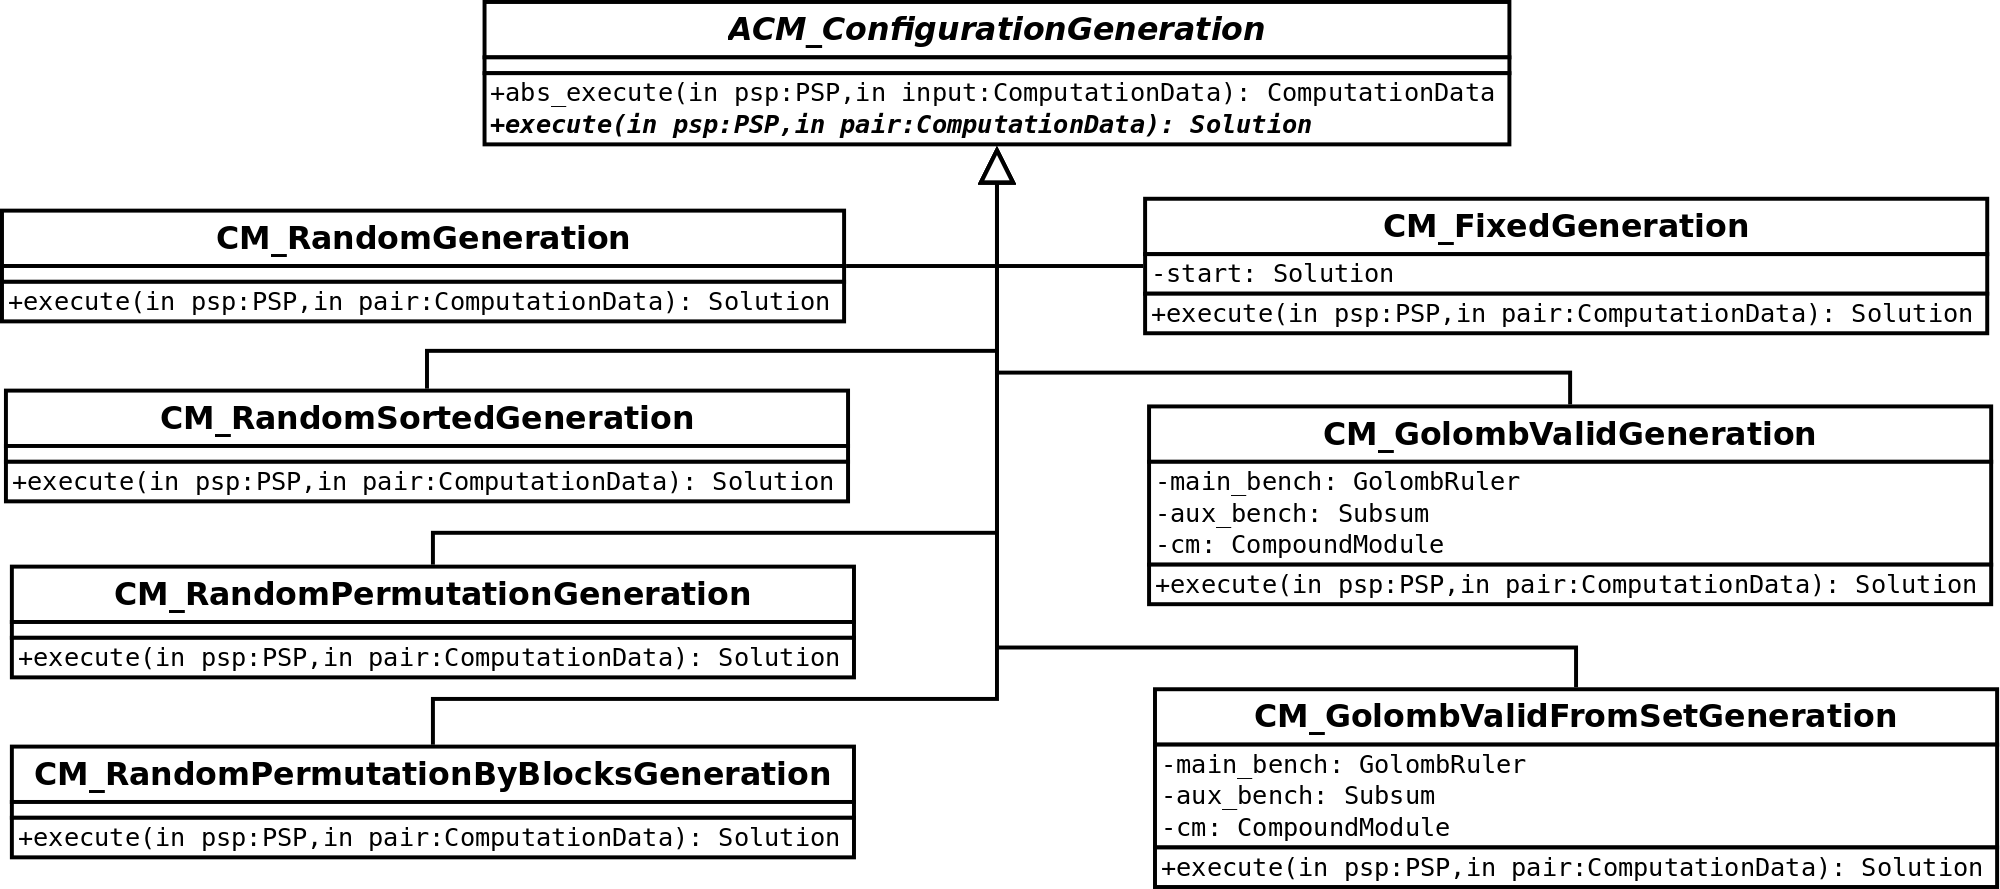
\includegraphics[width=\linewidth]{diaaomgen.png}
	\caption[]{Generation computation modules class diagram}\label{diag:genmodules}
\end{figure}

\begin{figure}
	\centering
	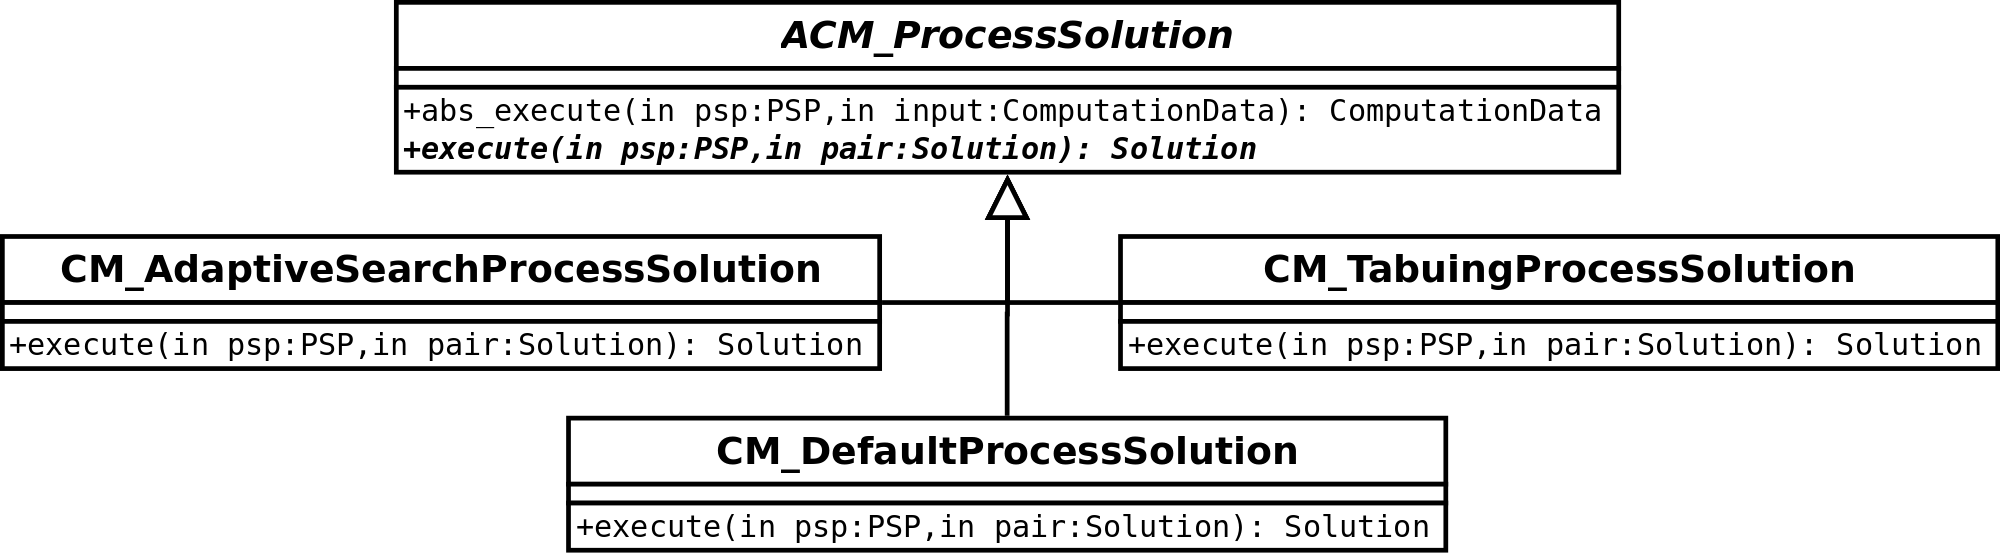
\includegraphics[width=\linewidth]{diaaomproconf.png}
	\caption[]{Processing solution computation modules class diagram}\label{diag:procconfmodules}
\end{figure}

\begin{figure}
	\centering
	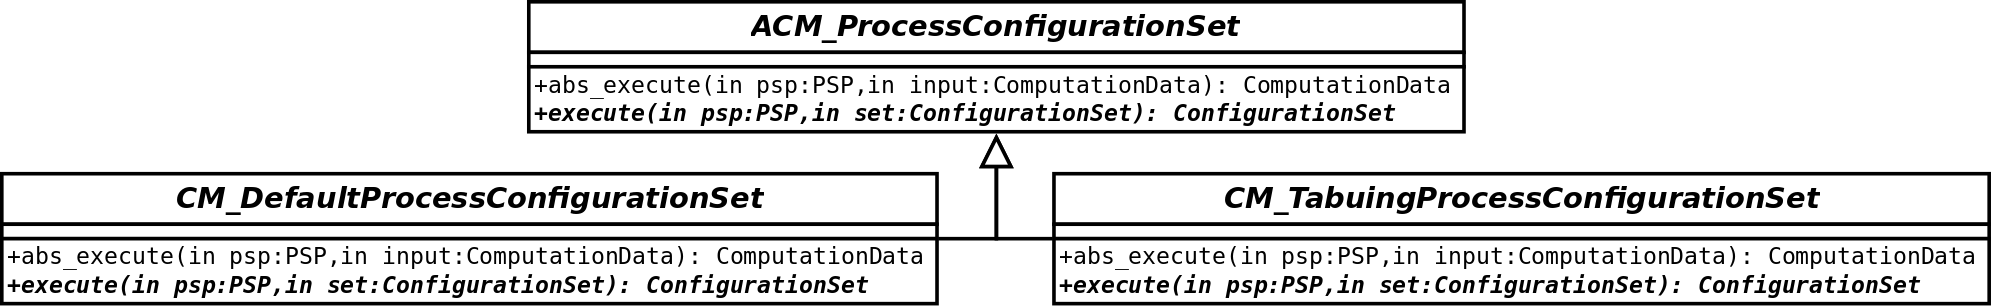
\includegraphics[width=\linewidth]{diaaomproset.png}
	\caption[]{Processing configuration--set computation modules class diagram}\label{diag:procsetmodules}
\end{figure}

\begin{figure}
	\centering
	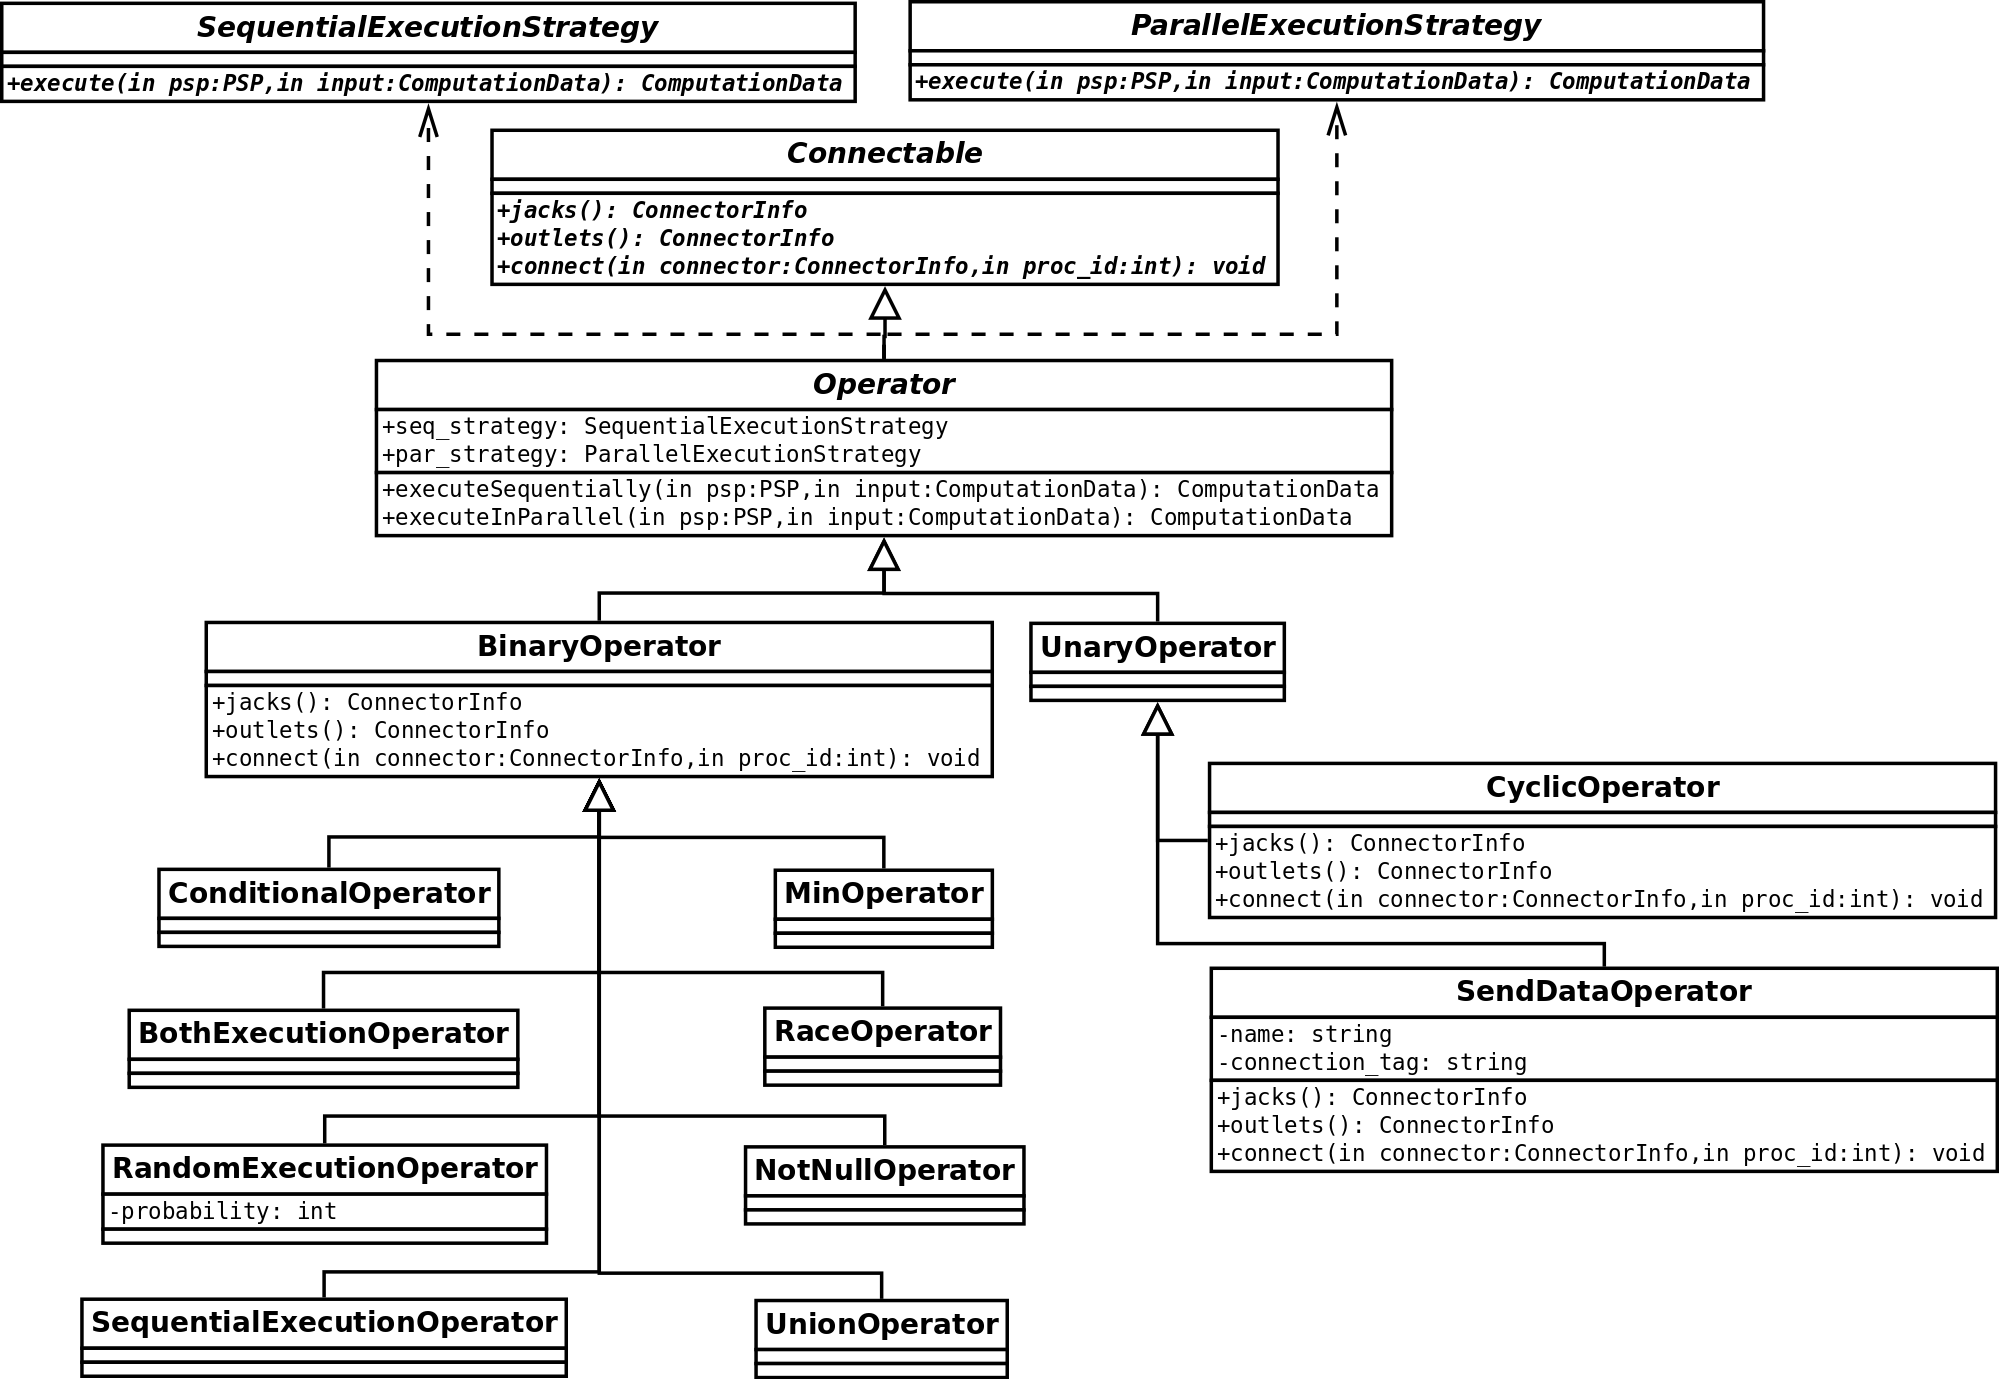
\includegraphics[width=\linewidth]{diaoperator.png}
	\caption[]{Operator class diagram}\label{diag:operator}
\end{figure}

\begin{figure}
	\centering
	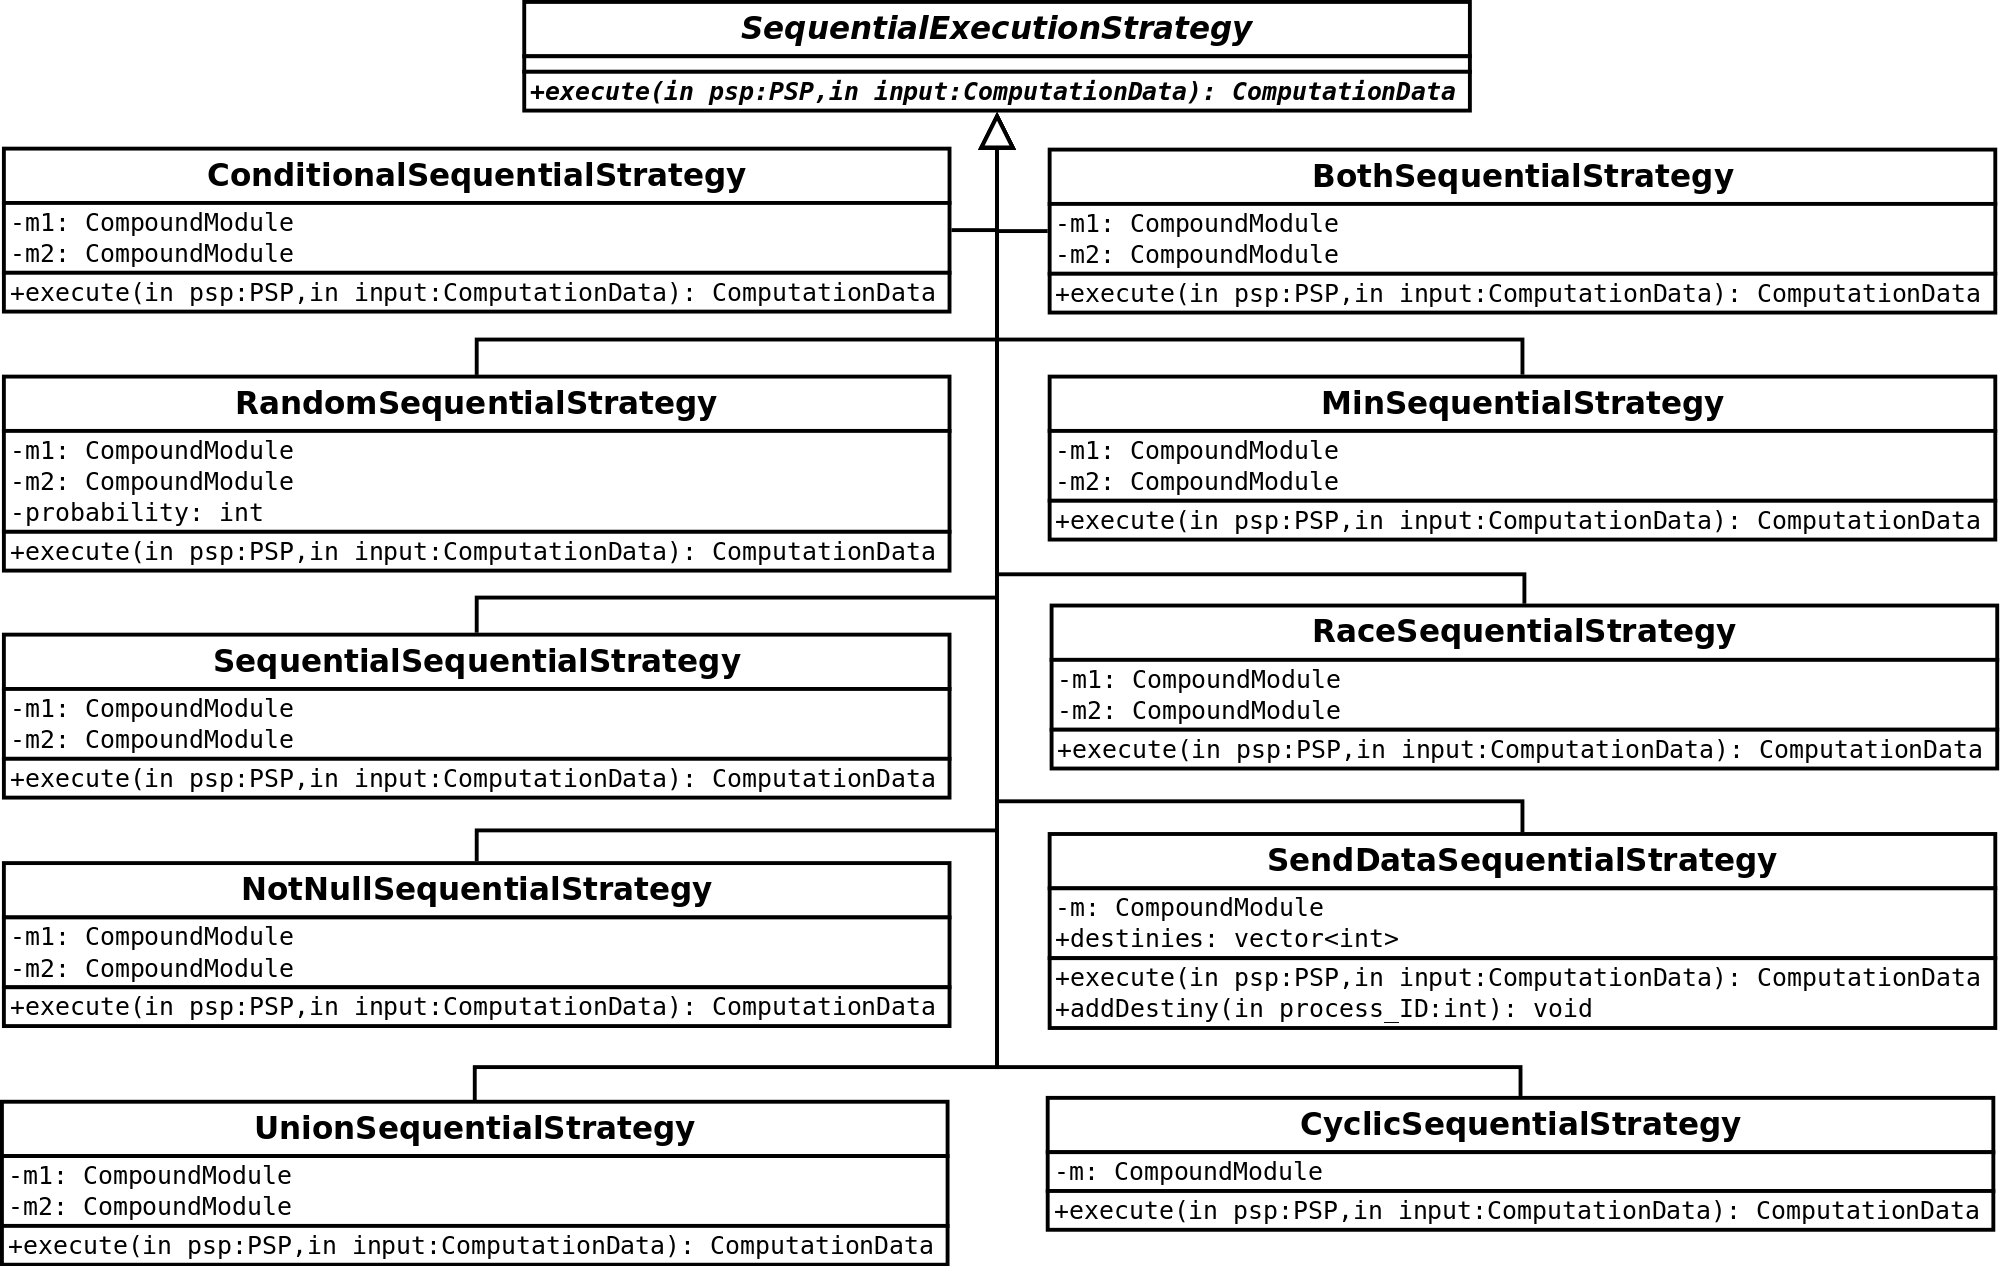
\includegraphics[width=\linewidth]{diaseqoper.png}
	\caption[]{Operator sequential strategy class diagram}\label{diag:seqoperstr}
\end{figure}

\begin{figure}
	\centering
	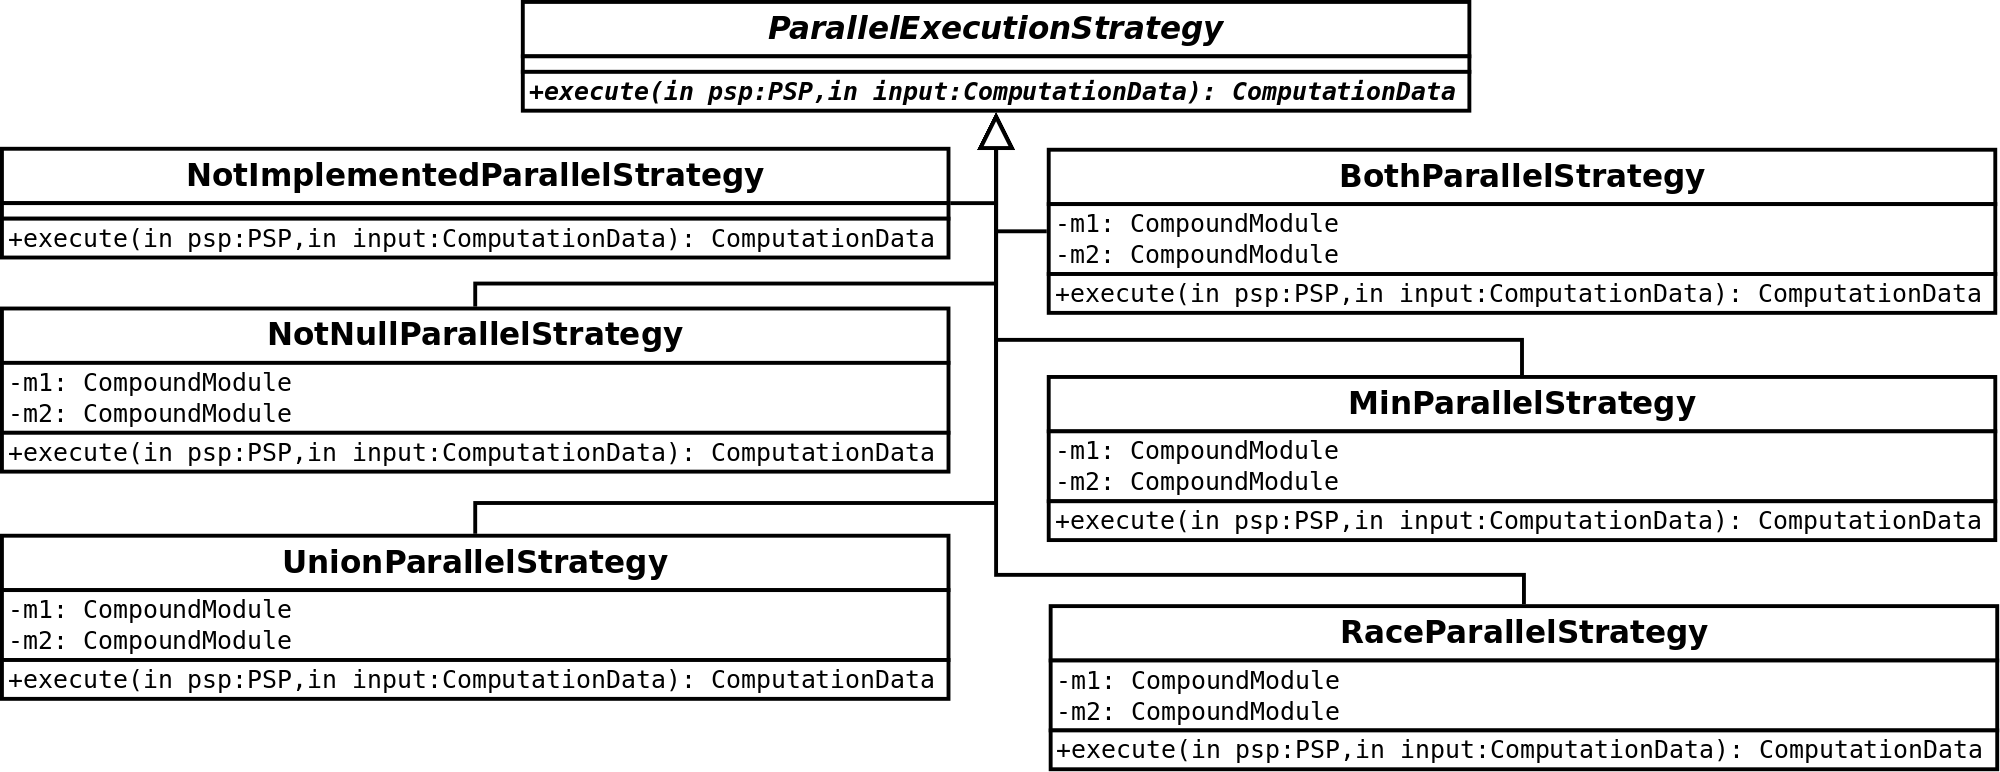
\includegraphics[width=\linewidth]{diaparoper.png}
	\caption[]{Operator parallel strategy class diagram}\label{diag:paroperstr}
\end{figure}

\begin{figure}
	\centering
	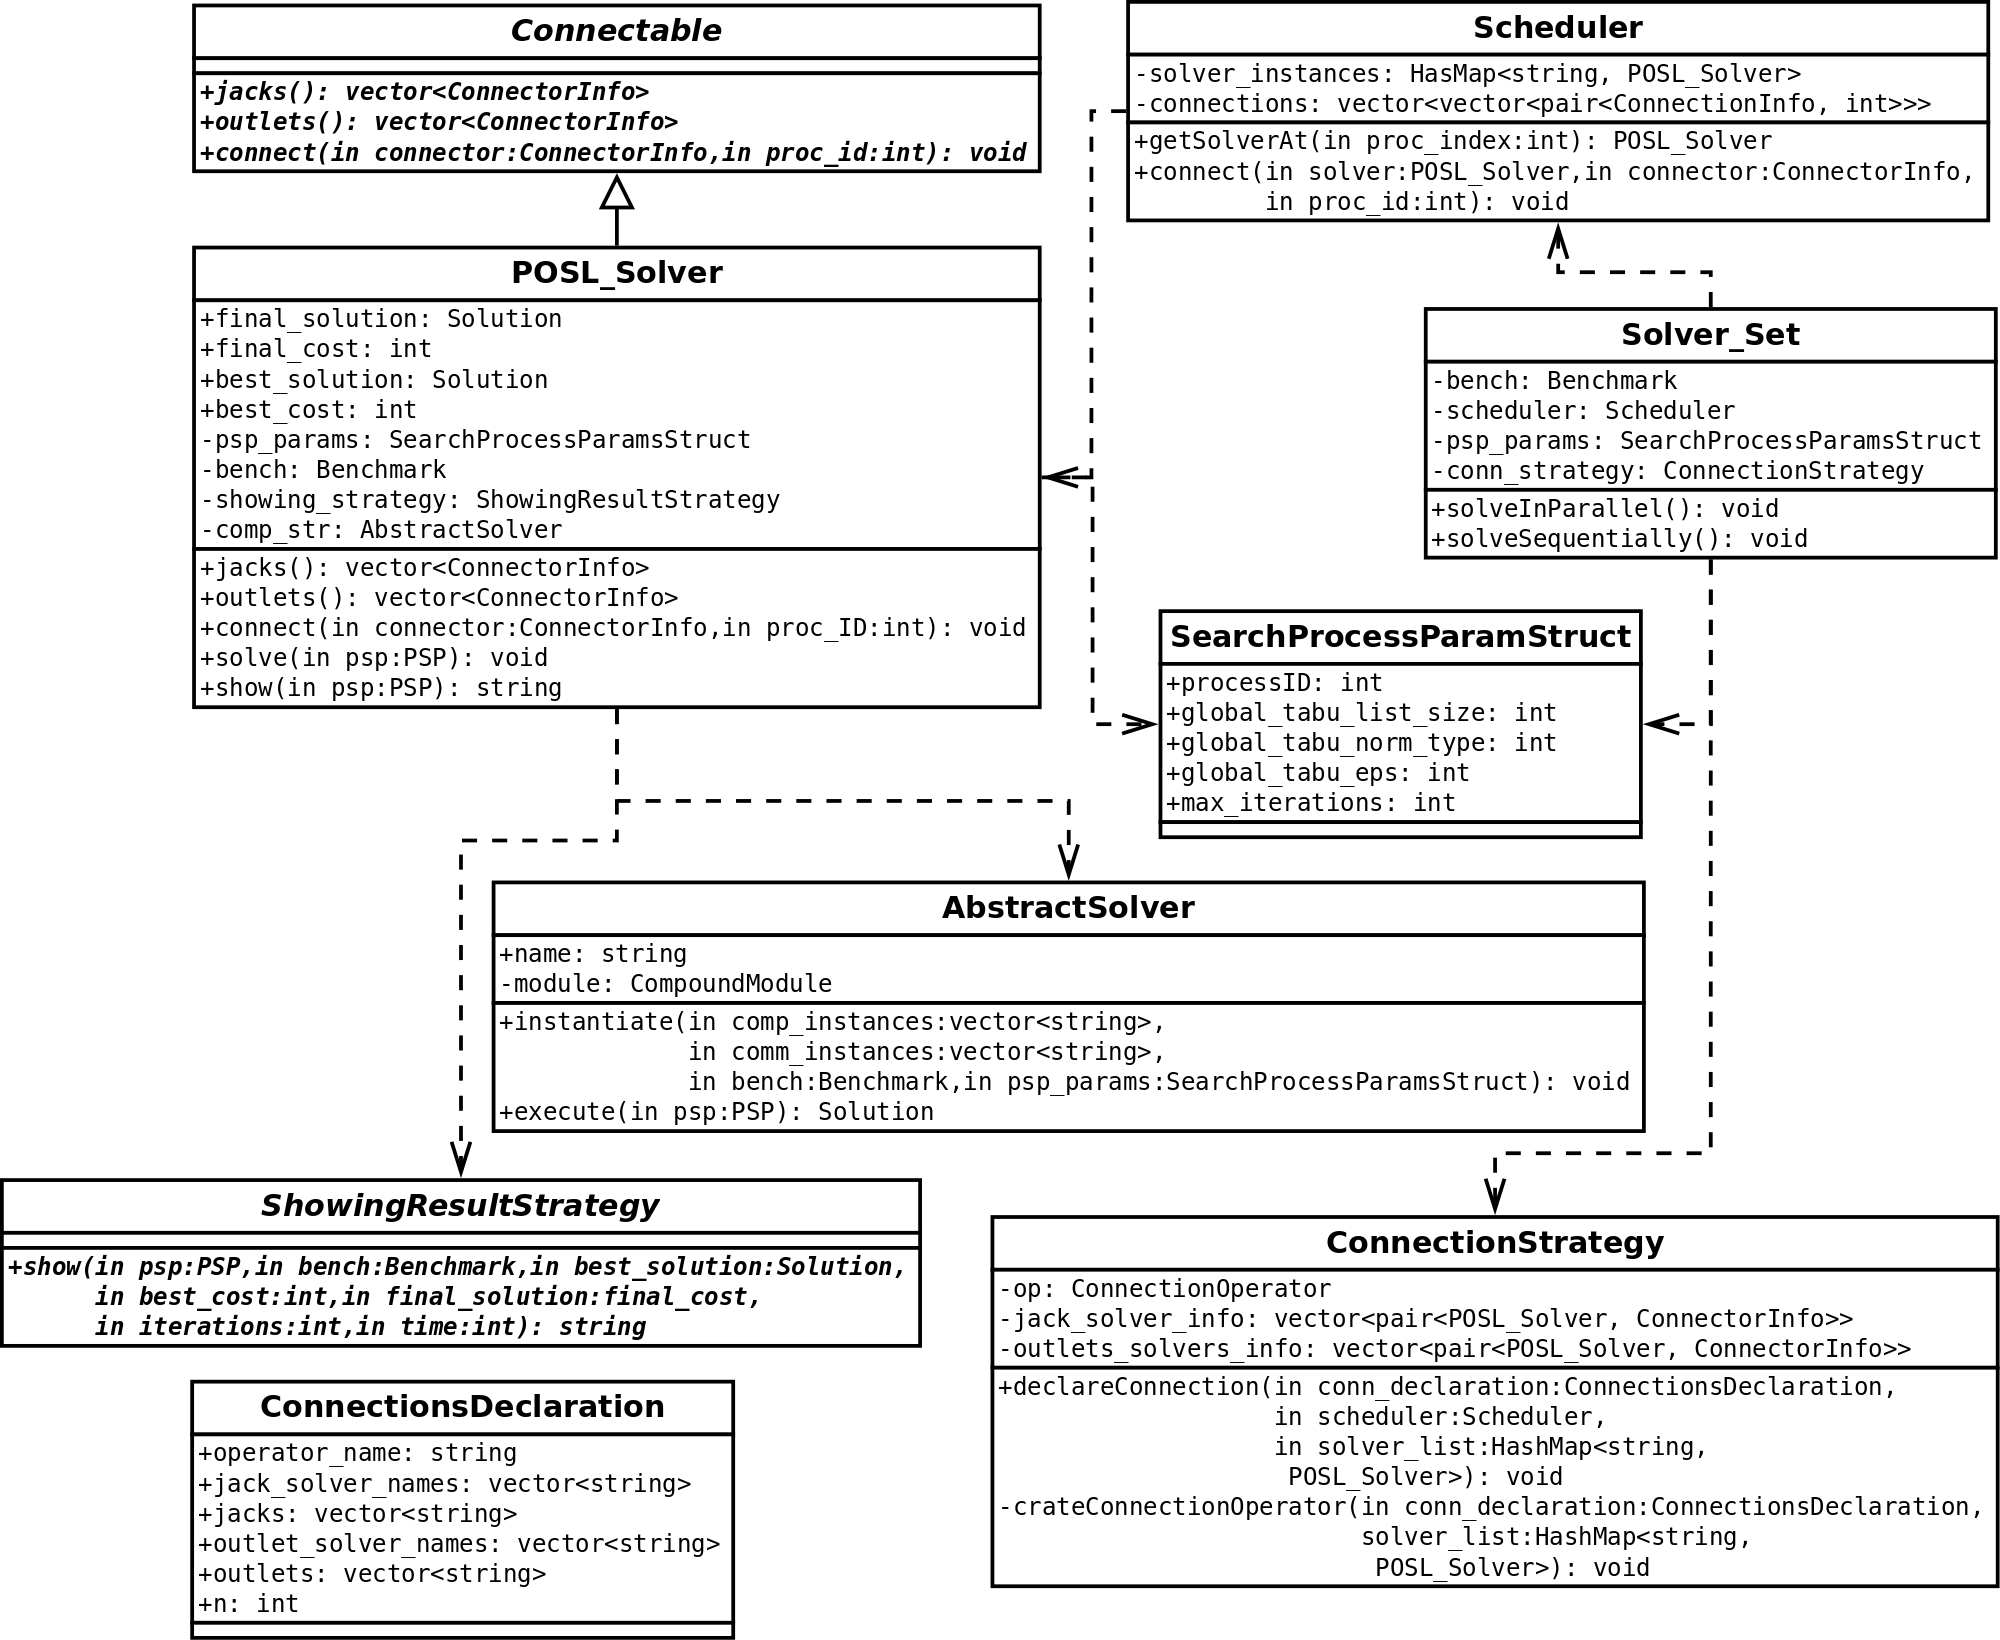
\includegraphics[width=\linewidth]{diasolverset.png}
	\caption[]{Solver Set class diagram}\label{diag:solverset}
\end{figure}

\clearpage 

\begin{figure}
	\centering
	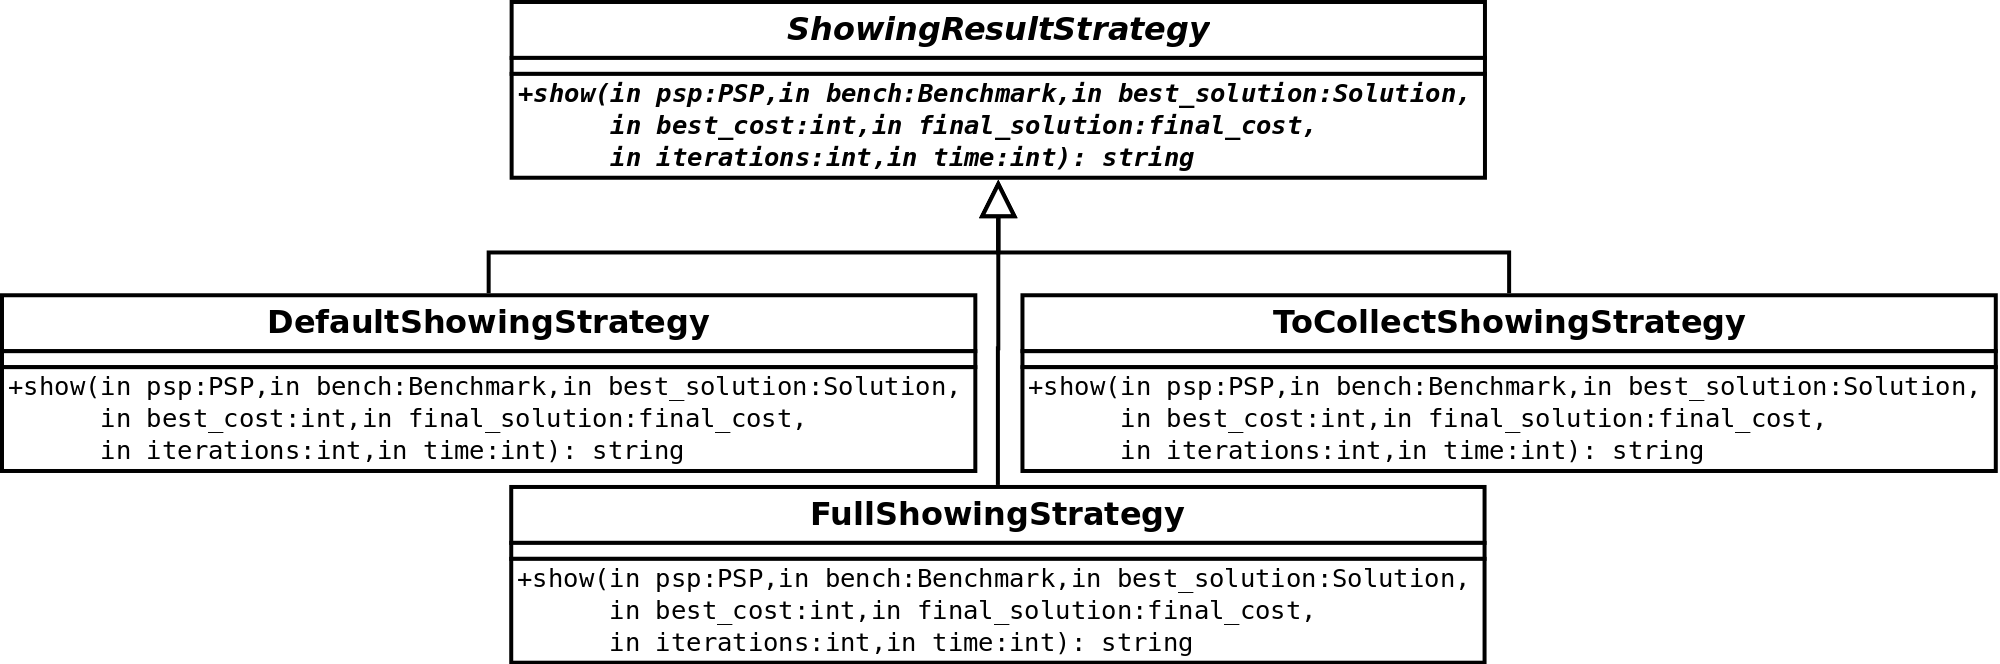
\includegraphics[width=\linewidth]{diaresultshowing.png}
	\caption[]{Showing result class diagram}\label{diag:showingres}
\end{figure}

\begin{figure}
	\centering
	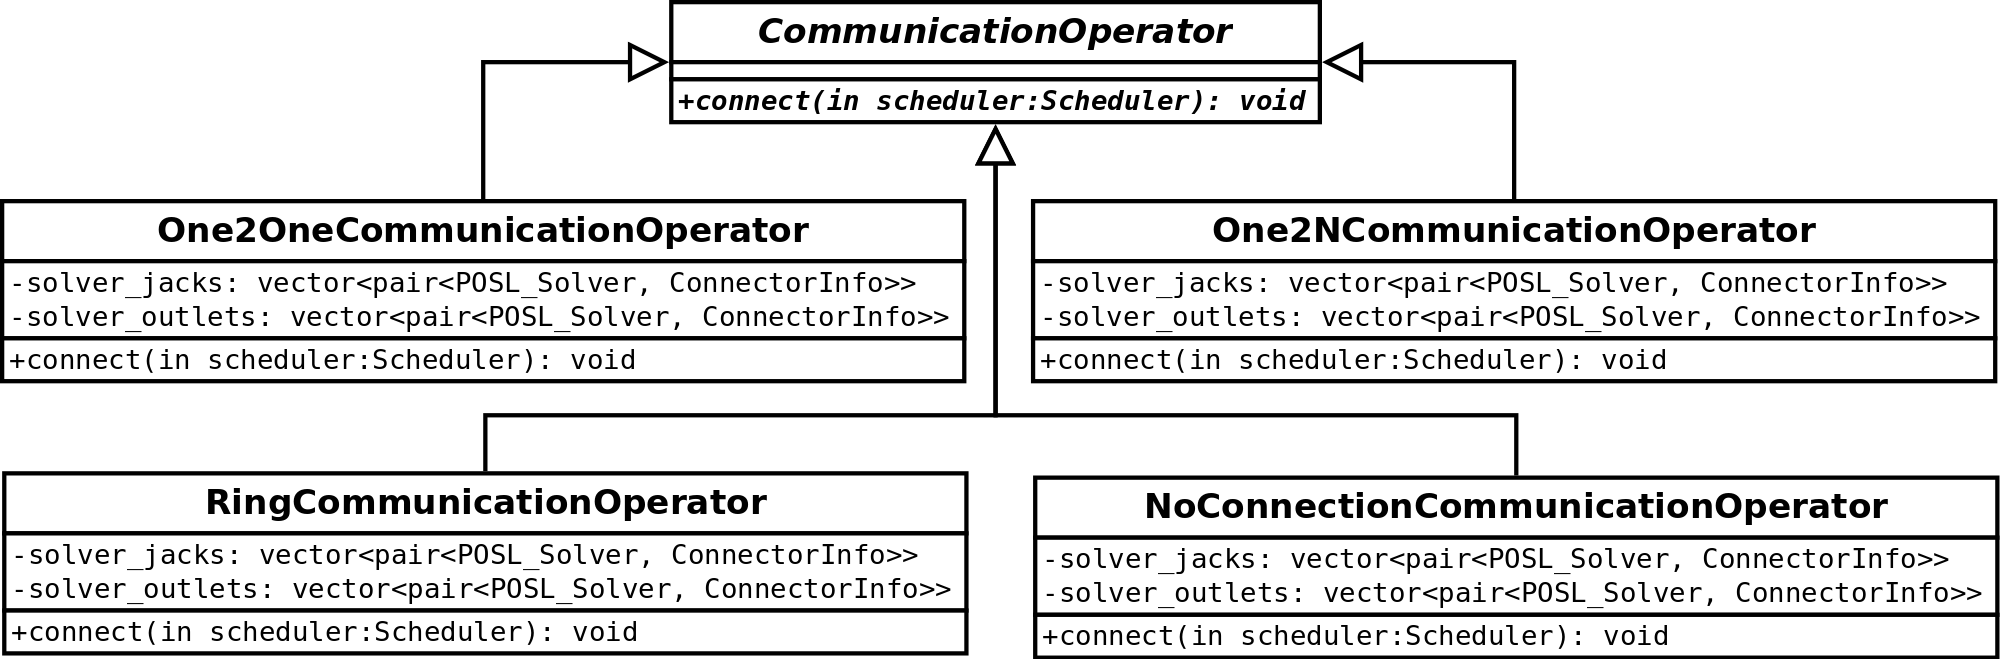
\includegraphics[width=\linewidth]{diacommoperator.png}
	\caption[]{Communication operator class diagram}\label{diag:commoper}
\end{figure}